% preamble:
\documentclass[12pt]{article}

\usepackage{amsmath,xcolor,todonotes,graphicx,marvosym,import,fullpage,textcomp,colortbl,array,pgfplots,lscape,soul,listings}

\definecolor{grey}{gray}{0.5}
\definecolor{lightgrey}{gray}{0.8}
\usepackage[numbers]{natbib}

%if you are annoyed of the colored boxes the hyperlinks in the pdf file uncomment this instead of the plain hyperref package above:
\usepackage[colorlinks=true, linkcolor=black, citecolor=black, urlcolor=black]{hyperref} 
\usepackage{NVC} %calles the style package NVC.sty created by Loes and Evert

%title infos
\date{\today}
\title{{\Huge Neurovascular Unit Model}\\
\vspace{2cm}
Documentation for Code ``OO-NVU Version 1.??''\\
{\large A merged NVC model of a neuron, astrocyte, smooth muscle cell, endothelial cell and the mechanical vessel response.
\vspace{7cm}}}


\author{by
Emiel van Disseldorp \and
Katharina Dormanns \and
Sanne van der Lelij \and
Joerik de Ruijter \and
Michelle Louise Goodman  \and
Eva Waldhauser \and
Moritz Burger \and
Kon Zakkaroff  \and
Tim David\footnote{Corresponding author, Tim.david@canterbury.ac.nz}}


%MATLAB code 
\usepackage[framed,numbered,autolinebreaks,useliterate]{mcode}

%Glossary
%\usepackage[
%nonumberlist, %do not show page numbers
%acronym,      %generate acronym listing
%toc,          %show listings as entries in table of contents
%section]      %use section level for toc entries
\usepackage{datatool}
\usepackage{glossaries}
\usepackage{hyperref}
\newglossary[slg]{symbolslist}{syi}{syg}{List of symbols} %Generate a list of symboles
\renewcommand*{\glspostdescription}{} %Remove the dot at the end of glossary descriptions
\makeglossaries %Activate glossary commands
\usepackage{glossary}

\pgfplotsset{compat=1.8}

%actual document:
\begin{document}
\maketitle
\newpage
\tableofcontents
\thispagestyle{empty}
\newlength\figureheight
\newlength\figurewidth

\section{Release notes}

\subsection{Changes to the previous version}

	\subsubsection{Astrocytic Calcium}
	
	\citet{Farr2011} implemented an NVU model based on a simple glutamate efflux into the SC simulating neuronal activity. This model included AC $Ca^{2+}$ variations induced by glutamate production into the SC and the subsequent efflux of $K^+$ into the PVS from a $Ca^{2+}$ mediated BK channel. In NVU 1.1 this BK channel was not \ca mediated and instead approximated by assuming a constant astrocytic \ca concentration.
			
	Although the model provided a qualitative description of neurovascular coupling the rate of change of $K_p$ was slow and the dilation of the associated arteriole took too long to reach even small dilations. The $K_p$ at which $v_i$ was maximally hyperpolarised was too high. 
	Therefore NVU version 1.1 did not contain any astrocytic $Ca^{2+}$ or glutamate input as the results were not satisfactory. 
	However various changes were implemented into the model and can be incorporated alongside the NO pathway, producing NVU version 1.2. 
	
	These changes included small fixes to the equations of the model by Michelle (e.g. changing a positive to a negative sign). 
	The additional state variables detailing the AC $Ca^{2+}$ model component are found in Table \ref{tab:NVU12ac}.
	
			\begin{table}[h!]
				\small
				\centering
					\begin{tabular}{c c l}
				\hline
				Variable & Unit & Description \\
				\hline
				$c_k$ & $\mu M$ & AC cytosolic $Ca^{2+}$ concentration \\
				$s_k$ & $\mu M$ & AC $Ca^{2+}$ concentration in the ER \\
				$h_k$ & - & inactivation variable denoting the action of $IP_3R$ that have not been activated by $Ca^{2+}$ \\
				$i_k$ & $\mu M$ & AC $IP_3$ concentration \\
				$eet_k$ &  $\mu M$ & $Ca^{2+}$ dependent EET production \\
				\hline
					\end{tabular}
					\caption{State variables related to $Ca^{2+}$ in the astrocyte}
					\label{tab:NVU12ac}
			\end{table}
			
	The ODE for astrocytic \ca is:
	\begin{equation}
	mklfmf
	\end{equation}
	
	\subsubsection{TRPV4 channel}
	
	Included is a transient receptor potential cation (TRPV4) channel on the astrocytic endfeet adjacent to the PVS.
	These channels are an important factor in astrocytic sensory and vasoregulatory functions as \cite{Dunn2013} have shown that certain TRPV4 channels can induce CICR in the endfeet of astrocytes and increase the strength of neurovascular coupling.
	The flux of $Ca^{2+}$ through the TRPV4 channel is based on the bidirectional model of \cite{Witthoft2012}.
	In this model vessel dilation activates the TRPV4 channels, allowing an influx of $Ca^{2+}$ from the PVS into the astrocytic cytosol. 
	The two additional state variables to the model are
	$m_k$: the open probability of the TRPV4 channel, and $c_p$: PVS $Ca^{2+}$ concentration (see Table \ref{tab:NVU12trpv4}).
			
					\begin{table}[h!]
						\small
						\centering
							\begin{tabular}{c c l}
						\hline
						Variable & Unit & Description \\
						\hline
						$c_p$ &  $\mu M$ & PVS $Ca^{2+}$  concentration (not in \cite{Farr2011}) \\
						$m_k$ & - & open probability of TRPV4 channel (not in \cite{Farr2011}) \\
						\hline
							\end{tabular}
							\caption{State variables related to the TRPV4 channel.}
							\label{tab:NVU12trpv4}
					\end{table}
					
			The ODE for the PVS \ca concentration is
				\begin{equation}
				\frac{d c_p}{dt} = - \frac{J_{TRPV_k}}{VR_{pa}} + \frac{J_{VOCC_k}}{VR_{ps}} - Ca_{decay_k} ( c_p - Ca_{min_k} ).
				\end{equation}
			
			Here $c_p$ always decays to the steady state value $Ca_{min_p}$ and $J_{VOCC_k}$ is a voltage operated calcium channel (VOCC) connecting the SMC to the PVS. When the membrane of the SMC hyperpolarises the channel closes. 
					
			The flux of \ca through the TRPV4 channel is:
				\begin{equation}
				J_{TRPV_k} = -\frac{1}{2} \frac{ G_{TRPV_k} m_k (v_k - E_{TRPV_k}) C_{correction} }{C_{astr_k} \gamma_k}
				\end{equation}
			
			The factor $1/2$ is there because there are 2 positive charges for every \ca ion \citep{Witthoft2013a}. 
			$E_{TRPV_k}$ is the Nernst potential of the TRPV4 channel:
				\begin{equation}
				E_{TRPV_k} = \frac{RT}{z_{Ca} F} \log \left(\frac{c_p}{c_k} \right).
				\end{equation}
			\\	
					
			The ODE for the open probability of TRPV4 channels is
				\begin{equation}
				\frac{d m_k}{dt} = \frac{m_{\infty_k} - m_k}{t_{TRPV_k}}.
				\end{equation}
						
			The equilibrium state of the TRPV4 channel is:
				\begin{equation}
				m_{\infty_k} = \frac{1}{1+\exp \left( {-\frac{\eta - epshalf_k}{\kappa_k}} \right) } 
								\frac{1}{1 + H_{Ca_k}} \left( H_{Ca_k} + \tanh \left( \frac{v_k - v_{1,TRPV}}{v_{2,TRPV}} \right) \right), 
				\end{equation}
			
			where $H_{Ca_k}$ is an inhibitory term:
				\begin{equation}
				H_{Ca_k} = \frac{c_k}{\gamma_{Cai}} + \frac{c_p}{\gamma_{Cae}},
				\end{equation}
			
			and $\eta$ is the local radial strain on the arteriole:
				\begin{equation}
				\eta = \frac{R - R_{passive}}{R_{passive}}.
				\end{equation}
			
			The strain on the perivascular endfoot of the AC is approximately equal to local radial strain on the arteriole since the endfoot surrounds the arteriole.	
			\\
				
			The flux of \ca through the TRPV4 channel is added to the AC \ca equation:
				\begin{equation}
				\frac{d c_k}{dt} = B_{cyt} \left( J_{IP3_k} - J_{pump} + J_{ER_{leak}} + \frac{\bm{{J_{TRPV_k}}}}{r_{buff}} \right). 
				\end{equation}
			
			The membrane potential of the AC is modified to include the TRPV4 channel:
				\begin{equation}
				\centering
				\scriptsize{
				v_k = \frac{g_{Na_k} E_{Na_k} + g_{K_k} E_{K_k} + \bm{g_{TRPV_k} m_k E_{TRPV_k}} + 
				                g_{Cl_k} E_{Cl_k} + g_{NBC_k} E_{NBC_k} + 		                g_{BK_k} w_k E_{BK_k} - 
				                J_{NaK_k} F / C_{correction}}{ g_{Na_k} + g_{K_k} + g_{Cl_k} + g_{NBC_k} + \bm{ g_{TRPV_k} m_k } + g_{BK_k} w_k }.
				           }
				\end{equation}
			
			The conductance $g_{TRPV_k}$ is calculated using the area of the astrocytic endfeet (similar to the calculation of the conductance of the BK channel at the astrocytic endfeet):
				\begin{equation}
				g_{TRPV_k} = \frac{G_{TRPV_k} 10^{-12}}{A_{ef_k}},
				\end{equation}
			
			where the conductance is multiplied by $10^{-12}$ to convert from $pS$ to $\Omega^{-1}$ (mho).
			
			The new parameters are found in Table \ref{tab:NVU12trpv4param}. 
			
			\begin{table}[h!]
				\small
				\centering
					\begin{tabular}{c c c l}
				\hline
				Parameter & Value & Unit & Description \\
				\hline
				$Ca_{decay_k}$ & 0.5 & - & Rate of decay of \ca in PVS \\
				$Ca_{min_k}$ & 2000 & $\mu$M & steady state value of \ca in PVS \\
				$t_{TRPV_k}$ & 0.9 & mV & Decay rate of the open probability $m_k$ \\
				$G_{TRPV_k}$ & 50 & pS & Conductance of TRPV4 channel \\
				$C_{correction}$ & $10^3$ & - & Convert from V to mV \\
				$C_{astr_k}$ & 40 & pF & AC cell capacitance \\
				$\gamma_k$ & 834.3 & mV $\mu M^{-1}$ & scaling factor relating movement of ions to membrane potential \\
				$epshalf_k$ & 0.1 & - & Strain required for half activation of the TRPV4 channel \\
				$\kappa_k$ & 0.1 & - & Related to strain and TRPV4 channel \\
				$v_{1,TRPV}$ & 0.12 & mV & Related to voltage gating of TRPV4 channel \\
				$v_{2,TRPV}$ & 0.013 & mV & Related to voltage gating of TRPV4 channel \\
				$\gamma_{Cai}$ & 0.01 & $\mu$M & Related to \ca concentration \\
				$\gamma_{Cae}$ & 200 & $\mu$M & Related to \ca concentration \\
				$r_{buff}$ & 0.05 & - & Rate of \ca buffering at the endfoot compared to the astrocyte body \\
				\hline
					\end{tabular}
					\caption{Model parameters related to the TRPV4 channel.}
					\label{tab:NVU12trpv4param}
			\end{table}
			
			Note that the flux of \ca through the TRPV4 channel is buffered at a lower rate $r_{buff}$, as the channel is located at the astrocytic endfoot and buffering is described by \cite{Witthoft2013} in the astrocytic soma. Therefore it is reasonable to assuming buffering at the smaller endfoot of the astrocyte will be at a lower rate. 
	
	\subsubsection{Nitric Oxide}
	
		Nitric oxide (NO) is a neurotransmitter known to act as a potent cerebral vasodilator. It is not produced in advance or stored and due its small size it is able to diffuse widely and readily in all 3 dimensions and is not limited to local effects, setting it apart from other signalling molecules of the central nervous system. It can rapidly spread even through membranes as it is extremely diffusible in aqueous and lipid environments. However NO has a very short half life as it is an unstable gaseous free radical, limiting its activity temporally \citep{Dobutovic2011} . 
					
		NO is produced in a variety of different tissues. The biochemical reaction that synthesises NO is catalysed by the enzyme family of nitric oxide synthases (NOS): neuronal (nNOS), endothelial (eNOS), and inducible (iNOS), found in neurons, ECs and multiple cell types respectively \citep{Forstermann2006}. 
		The literature suggests that the production source and quantity of NO determines its function; NO may either act neuroprotectively by controlling vascular smooth muscle tone and blood flow and hence preventing ischaemic cell injury, or neurotoxically leading to cerebral degeneration \citep{aurelia2010role}.
				
		The focus of the NO pathway is on NO production by nNOS and eNOS. Both enzymes' activation is mediated by intracellular $Ca^{2+}$ of the NE and EC respectively and eNOS is also activated by blood flow induced wall shear stress (WSS) in cerebral arterioles.
		NO is able to diffuse rapidly into other compartments. When NO reaches the SMC it interacts with intracellular enzyme activation and regulates SMC relaxation. 
		The dynamics of NO in the NE, AC, SMC and EC are described by using mass balance formulations. The NO concentration in compartment $j$ is:
			\begin{equation}
			\frac{d[NO]_j}{dt} = p_{NO,j} - c_{NO,j} + d_{NO,j}.
			\end{equation}
		$ p_{NO,j}$ is the production flux,  $c_{NO,j}$ is the consumption flux (i.e. reaction with oxygen or other molecules), and $d_{NO,j}$ is the diffusive flux. Diffusion is assumed to be linear with characteristic distance of $\Delta x = 3.75 \; \mu$m between the EC and SMC layers, and  $\Delta x = 50 \; \mu$m between the NE and SMC layers.
		The production rate is dependent on the concentration of activated NOS. nNOS and eNOS are thought to be the most influential NO producers, hence we assume NO production in only the NE and EC compartments and no production in the other cell types.
		
		NO synthesis in the NE is catalysed by nNOS in response to glutamate induced calcium influx into the post synaptic neuron and depends on the available concentration of the biochemical substrate L-Arginine (L-Arg) and oxygen ($O_2$). The nNOS activation is triggered by glutamate in response to neuronal activation. 
		NO production in the EC is catalysed by eNOS dependent on the availability of L-Arg and $O_2$ and is mediated by WSS. 
	
		NO, via its second messenger cGMP, influences the contraction of the SMC ($AMp$, $Mp$, $AM$, $M$) and the open probability of the SMC \pot channel $w_i$. NO activates soluble guanylyl cyclase (sGC) which catalyses the formation of cGMP. cGMP changes the rate constants $K_2$ and $K_5$ for the dephosphorylation of $Mp$ to $M$ and $AMp$ to $AM$ (these rate constant were previously set at $0.5 \; s^{-1}$ based on \citet{Koenigsberger2006}). $w_i$ is shifted to the left by cGMP via the equilibrium state $K_{act_i} (c_{w,i})$ with $c_{w,i}$ as a function of cGMP.
		\\
		
		The initial NVU model version 1.1 is extended into version 1.2 by additional mathematical equations that represent production, diffusion and consumption of NO in different cell types, as well as the interaction of NO with other biochemical species and ion channel open probabilities. The model of NVU 1.2 also contains astrocytic $Ca^{2+}$ and a TRPV4 channel. 		
		The additional NO pathway equations are found in the appendix of \cite{Dormanns2016} and corresponding additional state variables are detailed in Table \ref{tab:NVU12}. 		
		\todo[inline]{add equations here}

		\begin{table}[h!]
			\small
			\centering
				\begin{tabular}{c c l}
			\hline
			Variable & Unit & Description \\
			\hline
			$NO_n$ & $\mu M$ & NE NO concentration \\
			$NO_k$ & $\mu M$ & AC NO concentration \\
			$NO_i$ & $\mu M$ & SMC NO concentration \\
			$NO_j$ & $\mu M$ & EC NO concentration \\
			$cGMP$ & $\mu M$ & SMC cGMP concentration \\
			$eNOS$ & $\mu M$ & activated eNOS \\
			$nNOS$ & $\mu M$ & activated nNOS \\
			$c_n$ & $\mu M$ & NE cytosolic $Ca^{2+}$ concentration \\
			$E_b$ & - & fraction of sGC in the basal state \\
			$E_{6c}$ & - & fraction of sGC in the intermediate form \\
			\hline
				\end{tabular}
				\caption{State variables related to the NO pathway}
				\label{tab:NVU12}
		\end{table}
		

		Neuronal stimulation is simulated by an input of both glutamate and $K^+$ into the SC. The implementation of the NO pathway results in a larger steady state vessel radius, due to a constant supply of vasodilatory NO from the EC and NE. The radius profile also shows a larger and longer response to stimulation. 
		The response of the radius to stimulation can be divided into two components: the fast component in response to the SC $K^+$ increase (modelled by NVU version 1.1) and the slow component only found with the addition of the NO pathway. 
		
		The slower component of the model with the NO signalling pathway is the increase of cGMP in the SMC. This leads to the shift of the open probability of the SMC $K^+$ channel $w_i$. The  efflux of $K^+$ from the PVS increases with the opening of the channel so that the PVS $K^+$ concentration drops at a faster rate. Instead of reaching steady state conditions after around 100 s, as the model would do if the NO pathway is not included (version 1.1), the SMC membrane potential $v_i$ drops further. Consequently the VOCC channel closes further and the SMC $Ca^{2+}$ concentration decreases. As an overall behaviour the vessel dilates further and returns back to the resting state more slowly. 
		
		Hence the SC $K^+$ release governs the fast onset of vasodilation whilst the NO-modulated mechanisms (increase of SMC cGMP leads to shift in $w_i$) and the WSS activated NO release from the EC is responsible for maintaining the dilation longer and thus providing more oxygen and glucose to adjacent brain tissue with increased cerebral blood flow. In the resting state the EC provides the major contribution towards vasorelaxation, whereas during neuronal stimulation NO produced by the NE dominates \citep{Dormanns2016}.	
		
		The radius $r$ in this term is set as constant 25 $\mu m$ in order to create a reasonable boundary condition at the lumen side of the NVU based on physiological results.
		

\section{Code Structure}

The three core classes, the \texttt{Astrocyte}, \texttt{SMCEC} and \texttt{WallMechanics}, correspond to the components of the NVU model, namely the astrocyte model, the SMC and EC model, and the mechanical contraction cell model. For a given model component, all fluxes and ODEs are grouped together in the code of the corresponding class. The \texttt{NVU} class uses the three core component classes to collect the state variable and derivatives values and pass them to the \texttt{ode15s} solver for stiff problems. All classes in OO-NVU code are subclasses of the MATLAB's \texttt{handle} class which makes them appear as reference object to avoid unnecessary object duplication on assignment. Figure~\ref{fig:OO-Code-Structure} shows the public interfaces for all OO-NVU classes.

The following features apply to the \texttt{Astrocyte}, \texttt{SMCEC} and \texttt{WallMechanics} classes:

\begin{enumerate}
	\item The core classes rely on the class constructors to initialise the parameters with the help of the class-specific function \text{parse\_inputs(varangin)}. The constructors also initialise the variable indices, initial conditions and the output indices.
	
	\item In every core class the \texttt{rhs} method contains the algebraic and state variables, as well as the corresponding equations.
	
	\item The \texttt{shared(self, \~{}, u)} method, where present, provides the access to the shared algebraic or state variables used as input variables in the other model components where appropriate.
\end{enumerate}

\begin{figure}[htb!]
	\centering
	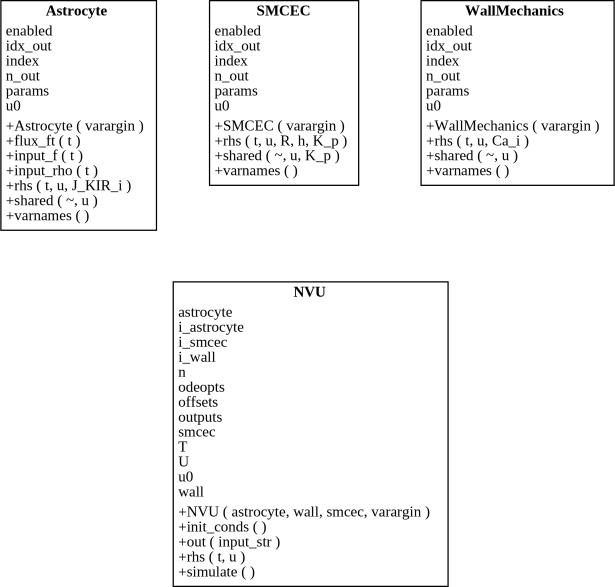
\includegraphics[width=0.7\linewidth]{figures/OO-Code-Structure}
	\caption[OO NVU Classes]{UML class diagram for the OO NVU code.}
	\label{fig:OO-Code-Structure}
\end{figure}

The code in the file \texttt{nvu\_script.m} provides a number of use-cases for running the NVU model. The code Listing~\ref{lst:NVU-Model-Init} shows an example of setting the options for the ODE solver \texttt{ode15s} specifying the \texttt{odeopts} parameter, however the code works well with default tolerances. The \texttt{simulate()} method of the \texttt{NVU} class start the simulation.

\begin{lstlisting}[language=Matlab,caption={Initialisation of the NVU model components.},label={lst:NVU-Model-Init},frameround=tttt,belowcaptionskip=10pt]
odeopts = odeset('RelTol', 1e-03, 'AbsTol', 1e-03, 'MaxStep', 1, 'Vectorized', 1);

nv = NVU(Astrocyte(), ...
WallMechanics(), ...
SMCEC('J_PLC', 0.18), ...
'odeopts', odeopts);

nv.simulate()
\end{lstlisting}



\section{Introduction}
\subsection{Neurovascular Unit}
%what cells do we look at and how are they orientated to each other? - take parts of L\&E

The cerebral cortex, a highly complex component of the human brain and part of the grey matter (\textit{substantia grisea}),   mainly consists of neurons (\gls{NE}s), unmyelinated axons and glial cells such as astrocytes (\gls{AC}s). It forms the outer layer of \textit{cerebrum} and \textit{cerebellum} and is veined with capillary blood vessels that provide the brain tissue with glucose and oxygen (\citet{Shipp2007}). These arterioles are surrounded by endothelial cells (\gls{EC}s) that form a thin layer on the interior surface of arterioles (\textit{intima}). The outer layer of the arteriole consists of smooth muscle cells (\gls{SMC}s), which are  aligned in circumferential direction. They define the contractile unit of the vessel and regulate its diameter by contraction and dilation.\\

A neurovascular unit (\gls{NVU}) defined in this research includes one cell of each of the described types and is graphically pictured in Figure~\ref{Overview1}. \\ 
\begin{figure}[h!]
  \centering
  \def\svgwidth{450pt}
  \scriptsize 
%  \includegraphics[width=130mm]{Bilder/Overview_NVU.png}
  \import{pics/}{Overview_without_gaps.pdf_tex}
  \caption{\textbf{Overview of different cells and domains that form a neurovascular unit.}  \gls{NE} - Neuron, \gls{SC} - Synaptic Cleft, \gls{AC}  - Astrocyte,  \gls{ER}  - Endoplasmic Reticulum,  \gls{PVS}  - Perivascular Space,  \gls{SMC}  - Smooth Muscle Cell, SR - Sarcoplasmic Reticulum,  \gls{EC}  - Endothelial Cell,     \gls{LU}  - Lumen with indicated blood flow. Intercellular communication via the exchange of ions is indicated by arrows. }
\label{Overview1}
\end{figure}

Each of the cell types and the spaces in between play an important role within the process of neurovascular coupling (\gls{NVC}, see Section \ref{section:NVC}). The synaptic cleft (\gls{SC}) is the space between an axon terminal and dendrite of two different \gls{NE}s in which neurotransmitters are released. It is enclosed by the star-shaped \gls{AC} that can take up released neurotransmitters. Protoplasmic \gls{AC}s are  polarized cells which can temporarily buffer extracellular \gls{K}, which is one of the key mechanisms within \gls{NVC}.  The astrocytic endoplasmatic reticulum (\gls{ER}), an isolated space in the cytosol, contains \gls{IP3}-sensitive \gls{Ca} channels, which can release \gls{Ca}-ions into the cytosol. The perivascular space (\gls{PVS}) is located between the end feet of an \gls{AC} and the arteriole. In the \gls{PVS}, ion exchange occurs between the arterial wall and the \gls{AC}.  The \gls{EC}s form a monolayer on the luminal side of the vessel in which all cells are aligned in the direction of the flow. It prevents passive diffusion of bigger molecules, while small ones, such as \gls{O2}, \gls{Ca} or \gls{IP3}, can pass through.  It also functions as an active organ sensing wall shear stress which plays an important role in the \gls{NO}-mediated pathway. Together with the SMC layer the endothelium forms the blood brain barrier (BBB), the physical frontier between brain tissue and blood vessel.
\gls{SMC} contraction occurs by actin and myosin filaments forming cross-bridges. The rate of contraction is dependent on the \gls{SMC} cytosolic \gls{Ca} concentration.
 






\subsection{Neurovascular Coupling} \label{section:NVC}
Neurovascular coupling (\gls{NVC}), or functional hyperaemia, describes the local vasodilation and~-contraction due to neuronal activation. The change in the vessel diameter (vasoreactivity) controls the blood flow and thereby the cerebral supply of oxygen and glucose.

Each cell type plays an important specific role during the process of NVC. Communication between cells is based on an exchange of ions through pumps and channels. These ion fluxes contribute to changes in cytosolic and intercellular species concentration and cell membrane potentials.

There are several pathways that can lead to vasocontraction or -dilation and are mediated by different signalling molecules, such as \gls{K}, \gls{Ca}, EET, \gls{NO} and 20-HETE. Neurotransmitters are released by the \gls{NE} into the \gls{SC} and can bind to receptors on dendrites of other neurons and astrocytes. This leads to a cascade of chemical reactions and the opening and closing of ion channels which influences the fluxes and concentrations.

%
%  be taken up by
%
% of events finally leading to inositol trisphosphate (IP3) production in the astrocytic cytosol [24].
% 
% 
% %  
%A change in the astrocyte’s membrane potential together with the increased EET concentration activates the BK-channels. These channels are located on the end-feet of the astrocyte and cause an efflux of K+ ions into the perivascular space. During neuronal activation this efflux increases.
%A moderate increase in the potassium concentration in the perivascular space causes the activa- tion of the potassium inward rectifying (KIR) channel. This KIR channel causes a depolarisation of the SMC. However, when the perivascular space’ potassium concentration is increased above a certain level, the KIR channel starts pumping potassium out of the cell, causing hyperpolarisation [2, 12].
%The voltage operated calcium channel (VOCC), which also interacts between SMC and its extra cellular space, pumps calcium into the cytosol. The influx of Ca2+ ions through the VOCC decreases when the SMC hyperpolarises [29] and amplifies the hyperpolarisation of the SMC.
%This hyperpolarasition decreases the influx of calcium. The calcium concentration in the SMC influences the myosin binding process. Actin filaments have several binding sites to which myosin can bind. However, in rest these binding sites are blocked by troponin. Free Ca2+ ions will cause troponin to move slightly which opens the binding sites. Then, cross bridges can be made between the actin and myosin. During hyperpolarisation, fewer Ca2+ ions enter the SMC. Consequentially, fewer cross bridges can be formed, which means that the vessel will dilate.
%A dilated vessel decreases the resistance to the flow, which causes an increase of flow and decrease of pressure drop over the vessel. Higher blood flow increases the diffusion process of chemicals, for example oxygen, through the cell wall into the surrounding tissue. Note that this is the intended response to neuronal activation of the NVU.
%
%%This document describes the code which includes the models of Ostby, Koenigsberger, HaiMurphy 


\subsection{Mathematical Approach}
The physiological models are based on a set of differential equations that describe the mass conservation of ions and molecules passing from one cell or domain to another. The simulations describe time-dependent ion fluxes and changes in membrane potential modelled by reaction rates that describe the kinetics which are physiologically validated by experimental data from the literature. This approach assumes homogeneous behaviour of a variable in a certain subdomain i.e. the spatial gradient of a variable in every subdomain is negligible.
%general mathematical modelling - definition of domains ('boxes') -  In the models  a lumped parameter approach is used.
%cells communicate with each other via ion fluxes - mathematically, this communication can be expressed by differential equations describing the mass conservation (explain!) and changes in membrane potential  

 


 
\section{Existing Models}

The present mathematical model is the first of its kind, leading the way in modelling the whole neurovascular coupling process. Starting with the neuronal activation we build up to the response in vessel diameter, utilizing all cell types and crucial pathways.  It is based on three existing models. 

\begin{itemize}
\item \textbf{The Astrocyte Model} - describes the crucial biochemical processes within the astrocyte (AC, \citet{Ostby2009}, reviewed  by \citet{LoesEvert}). 
\item  \textbf{The SMC and EC Model} - describes the behaviour and the main ion fluxes within the smooth muscle cell (SMC) and endothelium cell (EC). This model is based on that of \citet{Koenigsberger2006}. 
\item \textbf{The Contraction and Mechanical Model} -  describes the relationship between the cytosolic calcium (\gls{Ca}) concentration in the SMC and the contraction and dilation of the SMC by a myosin phosphorylation and cross-bridge based on the models of \citet{Hai1989} and Kelvin Voigt. \\
\end{itemize}

\subsection{The Astrocyte Model}
During neural activity, \gls{K} is released into the synaptic cleft (SC) by active neurons (NEs). In the astrocyte model, this is implemented by an influx of \gls{K} ($J_{K_s}$) with a corresponding \gls{Na} uptake by the neuron ($ J_{Na_s} $, Figure~\ref{fig:ACmodel}).
The increase of \gls{K} in the SC results in an increased \gls{K} uptake by the \gls{AC} which consequently undergoes depolarization. This results in a \gls{K} efflux from distant portions of the cell. Since most of the \gls{K} conductance of \gls{AC}s is located at the end-feet, the outward current-carrying \gls{K} would flow out of the cell largely through these locations. Consequently, the \gls{K} is 'siphoned' to the end-feet of the astrocyte and released into the perivascular space (\gls{PVS}) which leads to an increase of \gls{K} in the PVS. This \gls{K} release leads to a repolarization of the membrane voltage and is the input signal for the second (SMC \& EC) part of this model. \\

The AC model contains different types of active and passive ion channels. These ion channels and pumps are captured in a set of differential equations to describe the conservation of mass for the corresponding species concentrations in the SC, the \gls{AC} and the \gls{PVS}. The ion channels for potassium ($ J_{KCC1}$, $ J_{NKCC1} $, $ J_{K}$, $ J_{NaK} $ and $J_{BK}$), sodium ($ J_{NBC} $, $ J_{NKCC1} $,  $ J_{NaK} $ and  $ J_{Na} $), chloride ($ J_{KCC1}$, $ J_{NKCC1} $ and $ J_{Cl} $) and bicarbonate ($ J_{HCO_3}$) are included. Note that the bicarbonate and chlorine fluxes are coupled with the \gls{Na} and \gls{K} fluxes to obtain a neutral in- or efflux membrane voltage-wise.\\

The release of glutamate from the neuron in the synaptic cleft is simulated by creating a smooth pulse function $\rho$ that describes the ratio of bound to total glutamate receptors on the synapse end of the astrocyte. This induces an $IP_3$ release into the cell, causing the release of Calcium from the \gls{ER} into the cytosol, which then leads to the production of EET. The \gls{K} release into the \gls{PVS} is controled by the BK-channels. The opening of the BK-channels is regulated by the membrane voltage, as wel as the EET and \gls{Ca} concentration.
%\citep{Iadecola1993}. \\
\begin{figure}[h!]
  \centering
  \def\svgwidth{450pt} %400pt
  \scriptsize
  \import{pics/}{ACmodel_1pt1.pdf_tex}
  \caption{\textbf{Illustration of the astrocyte model.} All modelled fluxes are pictured, note that the indices (k - Astrocyte (AC), s - Synaptic Cleft (SC), p - Perivascular Space (PVS)) are left out for clarity reasons.}
\label{fig:ACmodel}
\end{figure}
\vspace{3cm}

\subsubsection{Input Signal}
In this model, a neuronal excitation was mimicked by an efflux of \gls{K} into the synaptic cleft (SC) and a simultaneous equal influx of \gls{Na} into the neuron from the SC (\citet{Ostby2009}, see equations in section \ref{sec:InputSignal}). The time-dependent input signal ($f(t)$, see figure \ref{fig:InputSignal}) starts at $t=200 s$ and ends at $t=210 s$. To estimate the profile $f(t)$ of the \gls{K} efflux/\gls{Na} influx, it is assumed that the \gls{K} efflux has a shape of a beta distribution with the governing parameters $\alpha$ and $\beta$ such that the profile is optimized according to two criteria \cite{Ostby2009}:\\
%
\begin{itemize}
\item [1.] The time from the start until the attaining maximum level of the \gls{K} concentration in the SC is 5s.
\item [2.] The level of the \gls{K} concentration in the SC at $ t = 30 $s is 60\% of the minimal level.
\end{itemize}
%
These two criteria take into account that $\beta$ is set at a value of $\beta = 5$.\\

In order to enhance the maximum \gls{K} level in the SC to reach the order of magnitude proposed by \citet{Filosa2004}, the amplitude of the input signal $f(t)$ is scaled up by the value $F_{input}$. The quantity of \gls{K} ions pumped into the AC can be derived by taking the integral of the flux $k_c f(t)$ over time, where $k_c$ is a constant that relates the input signal $f(t)$ to the \gls{K} influx. \\

The amount of released  ions are slowly buffered back by the neuron after the input signal terminates. This is modelled by a decay constant within the time interval $ 230 s \leq t \leq 240 s$. The integral of this block function is the same as the integral of the beta distribution in order to return to the baseline.\\

Beside this neuronal input signal, the NKCC1 and KCC1 co-transporters are only enabled when the neuronal ion release and spatial buffering are applied.  With both parameters added, the behaviour is modelled by a block function with the value $-F_{input}$ with a default value of zero (Figure \ref{fig:InputSignal}). \\
%
%
\begin{figure}[h!]
	\centering
	\footnotesize %not necessary
%	\newlength\figureheight 
%	\newlength\figurewidth 
	\setlength\figureheight{6cm} 
	\setlength\figurewidth{10cm}
%% 	\import{pics/}{InputSignal.tikz}
        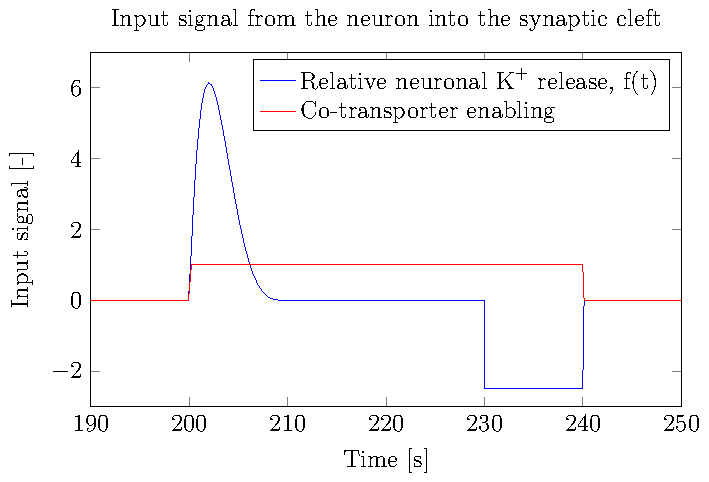
\includegraphics[width = 10cm]{pics/InputSignal.pdf}
	\caption{\textbf{The input signals used in the astrocyte model.} The \gls{K} efflux modelled by a beta distribution and buffered back afterwards (blue). The NKCC1 and KCC1 co-transporters are enabled when the neuronal ion release and spatial buffering is applied, modelled by a block function (red).  }
	\label{fig:InputSignal}
\end{figure}
% 
%
\subsubsection{Scaling}
The flux equations used in the AC model are based on the model of \citet{Ostby2009}. Their intention was to look at the volume changes of the AC and SC, therefore the volumes of both are variables in this model and all fluxes are scaled by a volume-surface ratio ($R_k$ and $R_s$, see Equations \ref{eq:R_k} and \ref{eq:R_tot}, respectively). It is assumed that the sum of the volumes of the AC and SC is a constant ($R_{tot}$). Due to osmotic pressure, the volume changes. We could show that the changes are comparatively small in our model and it would be justifiable to leave out the scaling factors. However, at the moment they are included because the given fluxes of \citet{Ostby2009} are scaled by the volume-surface ratio. It should be considered in future versions to eliminate the scaling factors by multiplying the fluxes with an adequate constant. 




\subsection{SMC and EC Model}
The SMC and EC model is based on the work of \citet{Koenigsberger2006}, see Figure~\ref{fig:SMCECmodel}. This model is extended by adding an inward-rectifier potassium (KIR) channel in the SMC ($ J_{KIR} $, \cite{Filosa2004}) in order to create a connection between the Astrocyte model and the SMC and EC model. \\%A conservation of \gls{K} was added in the SMC and EC model  for the PVS and SMC.\\

The input signal for this model is the \gls{K} concentration in the PVS which is increased by the efflux of astrocytic potassium after neuronal activity. 
\begin{figure}[h!]
  \centering
  \def\svgwidth{450pt} %400pt
  \scriptsize
  \import{pics/}{SMCECmodel3.pdf_tex}
  \caption{\textbf{Illustration of the SMC and EC model.} All modelled fluxes are pictured, note that the indices (k - Astrocyte (AC), s - Synaptic Cleft (SC), p - Perivascular Space (PVS)) are left out for clarity reasons.}
\label{fig:SMCECmodel}
\end{figure}

The raise in \gls{K} in the PVS activates the KIR channel on the SMC, causing them to open extruding more potassium into the PVS. This efflux of \gls{K} hyperpolarizes the SMC membrane and causing the voltage-operated \gls{Ca} channels to close, preventing the influx of \gls{Ca} into the SMC cytosol.\\

The cytosolic \gls{Ca} concentrations in the SMC and EC and that in the sacroplasmatic reticulum (SR) and endoplasmatic reticulum (ER), respectively, are described by a set of differential equations. In- and effluxes  of \gls{K} are given by the following ion channel and pumps: $ J_{KIR} $, $ J_{NaK} $ and $ J_{K} $. \gls{Ca} leaves the SR via the channels: $ J_{CICR} $, $ J_{IP_3} $ and $ J_{SR\_leak} $ and enters it by $ J_{SR\_upt} $. The in- and efflux of \gls{Ca} are modelled with $ J_{extr} $, $ J_{VOCC} $, $ J_{stretch} $ and $ J_{NaCa} $. Note that these fluxes link the cytosol with the extracellular matrix. Here again, a chloride pump is included, $ J_{Cl} $, to return to the resting membrane potential.\\

Physiologically, ECs and SMCs are connected by gap junctions that allow an intercellular exchange of molecules and voltage.  \citet{Koenigsberger2006} include the coupling factors $J_{Ca^{2+}-cpl}^{EC-SMC}$, $V_{cpl}^{EC-SMC}$ and $J_{IP_{3}-cpl}^{EC-SMC}$ for \gls{Ca}, voltage and IP$ _3 $ coupling, respectively. The strength of the coupling can be changed in the code with the variable $ CASE $.\\

Inositol triphosphate (\gls{IP3}) is an important messenger molecule. It's production, in the endothelium, is triggered by agonist binding onto membrane receptors. IP$_3$ mediates the $ J_{IP_3} $ channel, situated between the reticulum and cytosol. 
The production rate of IP3 is a constant over time and can be changed by altering the variable  $ J_{PLC}$ within the mathematical model .\\

Note that the model of \citet{Koenigsberger2006} already includes \gls{Ca}-buffering in the SMC and EC.







%\todo[inline]{What is the expected PLC agonist concentration in the EC?}
%\begin{itemize}
%\item based on \cite{Koenigsberger2006} with a KIR channel added
%\item \todo[inline]{rho as a buffering factor should be added (equation from \cite{Gonzalez1994})}
%\item coupling between EC and SMC included (voltage, Ca, IP3)
%\item \todo[inline]{include stretch activated channels}
%\item the only link between AC model and this model is the potassium efflux through the KIR channel  
%\item \todo[inline]{Potassium conservation of mass equation needs to be included}
%\item Do the NaK pump and the Ki channel lead into the PVS ? (at the moment into nowhere)
%\end{itemize}



%\todo[inline]{Tim's question: Should Ca coupling be included in the membrane potential equation? at the moment there is a voltage coupling, but we want to include also the Ca coupling in the membrane potential equation}

\subsection{Contraction and Mechanical Model}

\subsubsection{Contraction Model}
The contraction and mechanical part of the model is based on the model of \citet{Hai1989}, which describes the formation of cross bridges between the myosin and actin filaments (Figure~\ref{fig:MechModell}). This is coupled with a Kelvin-Voigt model that is used to describe the visco-elastic behaviour of the arterial wall (Figure~\ref{fig:KelvinVoigt}).\\
\begin{figure}[h!]
  \centering
  \def\svgwidth{450pt} %400pt
  \footnotesize
  \import{pics/}{MechanicalModel.pdf_tex}
  \caption{\textbf{Illustration of the contraction model within the smooth muscle cell. }}
\label{fig:MechModell}
\end{figure}

The \gls{Ca} concentration in the SMC is the input signal for the cross bridge model of \citet{Hai1989}. The model uses four possible states for the formation of myosin: free nonphosphorylated cross bridges (M), free phosphorylated cross bridges (Mp), attached phosphorylated cross bridges (AMp) and attached dephosphorylated latch bridges (AM). The dynamics of the fraction of myosin in a particular state is given by four differential equations.\\

The active stress of the SMC is directly proportional to the fraction of attached cross bridges (AM and AMp). Using this model the relation between the cytosolic \gls{Ca} concentration and the active stress of the SMC can be derived.\\

\subsubsection{Mechanical Model}
The fraction of attached myosin cross bridges is the input signal for the visco-elastic mechanical model (Kelvin Voigt, Figure~\ref{fig:KelvinVoigt})  which describes the changes in radius over time. The pressure inside the vessel wall is taken as a constant and the circumferential stress is calculated using the Laplacian law. 


\begin{figure}[h!]
  \centering
  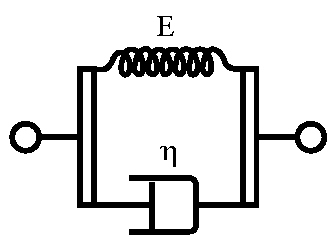
\includegraphics[width = 5 cm]{pics/Kelvin_Voigt_diagram.pdf}
  \caption{\textbf{Schematic overview of a Kelvin Voigt model.}}
  \label{fig:KelvinVoigt}
\end{figure}

The Young's modulus and initial radius of the vessel wall is divided into an active and a passive part and is a function of the attached myosin cross-bridges. The active and passive Young's modulus are based and fitted on experimental data of \citet{Gore} which is shown in Figure~\ref{fig:LinearisationRadius}. 

\begin{figure}[h!]
  \centering
  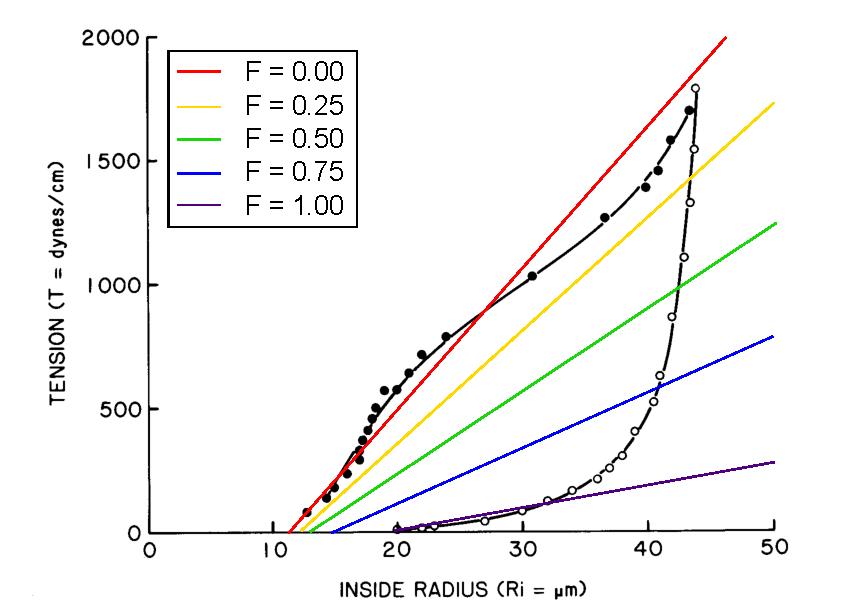
\includegraphics[width = 12 cm]{pics/LinearisationRadius.pdf}
  \caption{\textbf{Linearisation for the Young's modulus and initial radius on the data of \citet{Gore} for different values of F.}}
  \label{fig:LinearisationRadius}
\end{figure}

Figure~\ref{fig:LinearisationRadius} shows that the initial radius ($R_0$) decreases when the fraction of attached myosin cross bridges (F) are increased (the intersection with the x-axis). The figure also shows that the Young's modulus, represented by the slope of the lines in the tension-strain graph, increases when F increases. The linearisations of the Young's modulus can be described by:
\begin{equation} \label{eq:Fbalans4}
T=\frac{\Delta T}{\Delta R}(R-R_0)~,
\end{equation}
where $T$ is the tension of the vessel and $\frac{\Delta T}{\Delta R}$ is the slope of the linearisations in Figure~\ref{fig:LinearisationRadius}. \\

%Gore and Davis et al.\\
\newpage
\subsection{Merging of All Models}

The Astrocyte model and the \gls{SMC} and \gls{EC} model are linked by the SC and the \gls{PVS}. The \gls{K} input signal of the neuron is pumped into the \gls{SC} and taken up afterwards by the AC. The most important ion pumps and channels in this process are the \gls{K} channels in the neuron which releases the \gls{K} input,  the \gls{Na}/\gls{K} pump and \gls{K} channel in the \gls{AC} which pump the released \gls{K} into the AC.
The result of this is an efflux of \gls{K} at the end feet of the astrocyte using the BK-channel. Consequently, the membrane voltage of the astrocyte re-polarizes and the \gls{K} concentration in the PVS increases. This increased \gls{K} concentration activates the KIR channel in the \gls{SMC} and start to pump out more \gls{K} from the \gls{SMC} into the \gls{PVS}. The increased efflux of \gls{K} hyperpolarises the \gls{SMC} membrane voltage and as a result of that the VOCC closes and prevents the influx of \gls{Ca} into the \gls{SMC}.
Summarising, the neuronal input signal leads to a decrease of \gls{Ca} influx by the VOCC channels and therefore a decrease of the intracellular \gls{Ca} concentration. This leads to a decreased fraction of attached myosin bridges in the \citet{Hai1988} model, resulting in vessel dilation in the visco-elastic mechanical model. An overview of the whole model is shown in Figure~\ref{Overview}.

\begin{figure}[h!]
  \centering
  \def\svgwidth{450pt}
  \scriptsize 
  \import{pics/}{All_models_1pt1.pdf_tex}
  \caption{\textbf{All Models.}}
\label{Overview}
\end{figure}






%\begin{itemize}
%%\item What is the real relationship between the Ca concentration and the radius? - more references needed!
%%\item At the moment: Ca input of SMC, cross-bridge model of \citet{HaiMurphy}, Kelvin-Voigt model for elastic response of the arterial wall (assuming Laplace-law), change in radius 
%\end{itemize}


%\documentclass[12pt]{article}
%\usepackage{amsmath,xcolor,todonotes,graphicx,marvosym,dsfont,import,fullpage,textcomp,colortbl,array,pgfplots,lscape}
%\begin{document}
	\section{Results}
	\subsection {OO-NVU 2.0}
	\subsubsection*{Potassium input signal (figure \ref{fig:1IS})}
	At the top the neuronal \gls{K} input signal is shown. This input signal is pumped into the SC by the \gls{NE}. As a result of that, there is more \gls{K} taken up by the \gls{AC} in the beginning of the input pulse, and released at the end of the input pulse. In the second graph the membrane potential of the AC is shown over time. When the \gls{K} concentration in the SC is increased the membrane voltage depolarises and when the \gls{K} concentration in the SC decreases the membrane potential repolarises again.
	In the third graph the fluxes into the PVS are shown. In blue the flux by the astrocytic BK channel, and in green the flux by the KIR channel in the SMC is shown. The drop in the middle of the KIR flux is caused because the SMC becomes in a oscillatory state and therefore the efflux by the KIR channel follows the \gls{Ca} waves inside the SMC.
	The bottom figure shows the \gls{K} concentration in the PVS.
	
	\subsubsection*{Neurovascular Coupling Overview (figure \ref{fig:1})}
	This figure describes the main pathway from the synaptic cleft to the radius change. It starts with a \gls{K} concentration in the synaptic cleft, followed by the flux trough the BK-channel determined in the astrocyte, leading to an increased \gls{K} concentration in the perivascular space. This causes an increased  \gls{K} influx trough the KIR channel, changing the membrane voltage of the SMC. The \gls{Ca} flux through the VOCC increases, decreasing the \gls{Ca} concentration in the SMC and thereby inducing vasodilation. 
			
	
	\subsubsection*{AC State Variables (figure \ref{fig:2})}
	The graphs display the concentrations of \gls{K}, \gls{Ca}, Cl and HCO3 in the astrocyte and \gls{K} in the SC and PVS. These concentrations, together with the membrane voltage contribute to the opening of the BK-channel in their own way. The open state of the BK channel determines the potassium flux from the astrocyte to the perivascular spcace, where it induces vascular contraction.
	
	\subsubsection*{AC Fluxes (figure \ref{fig:3})}
	All ion fluxes that enter or leave the astrocyte.
	
	
	\subsubsection*{SMC EC State Variables and Coupling (figure \ref{fig:4})}
	The graphs in this figure shows the solutions of the differential equations of the \gls{SMC} and \gls{EC}, including the intracellular \gls{Ca} concentration, the \gls{IP3} concentration, the sarcoplasmic (\gls{SMC}) or endoplasmic (\gls{EC}) \gls{Ca} concentration, the membrane voltage and the coupling fluxes between EC and SMC.
	
	\subsubsection*{SMC Fluxes (figure \ref{fig:5})}
	In these figures the coupling and the fluxes in the SMC are shown. When one of the fluxes is negative, it means that the direction of the flux is in the opposite than it is defined in the equations. These figures show that when the neuronal signal is given, the VOCC closes and that the SMC contracts. 
	
	\subsubsection*{EC Fluxes (figure \ref{fig:6})}
	All ion fluxes that enter or leave the EC.
	
	\subsubsection*{Contraction Model and Radius (figure \ref{fig:7})}
	In this figure the fraction of the four states (M, Mp, AMp, AM) of myosin in the SMC are shown at the top. At the bottom left the fraction of attached cross bridged myosin (the sum of AM and AMp) is shown. And at the bottom right the radius is plotted over time. The increase in vessel diameter is in the expected order of magnitude.
	
	
	\begin{landscape}
			
		\begin{figure}[h!]
			\centering
			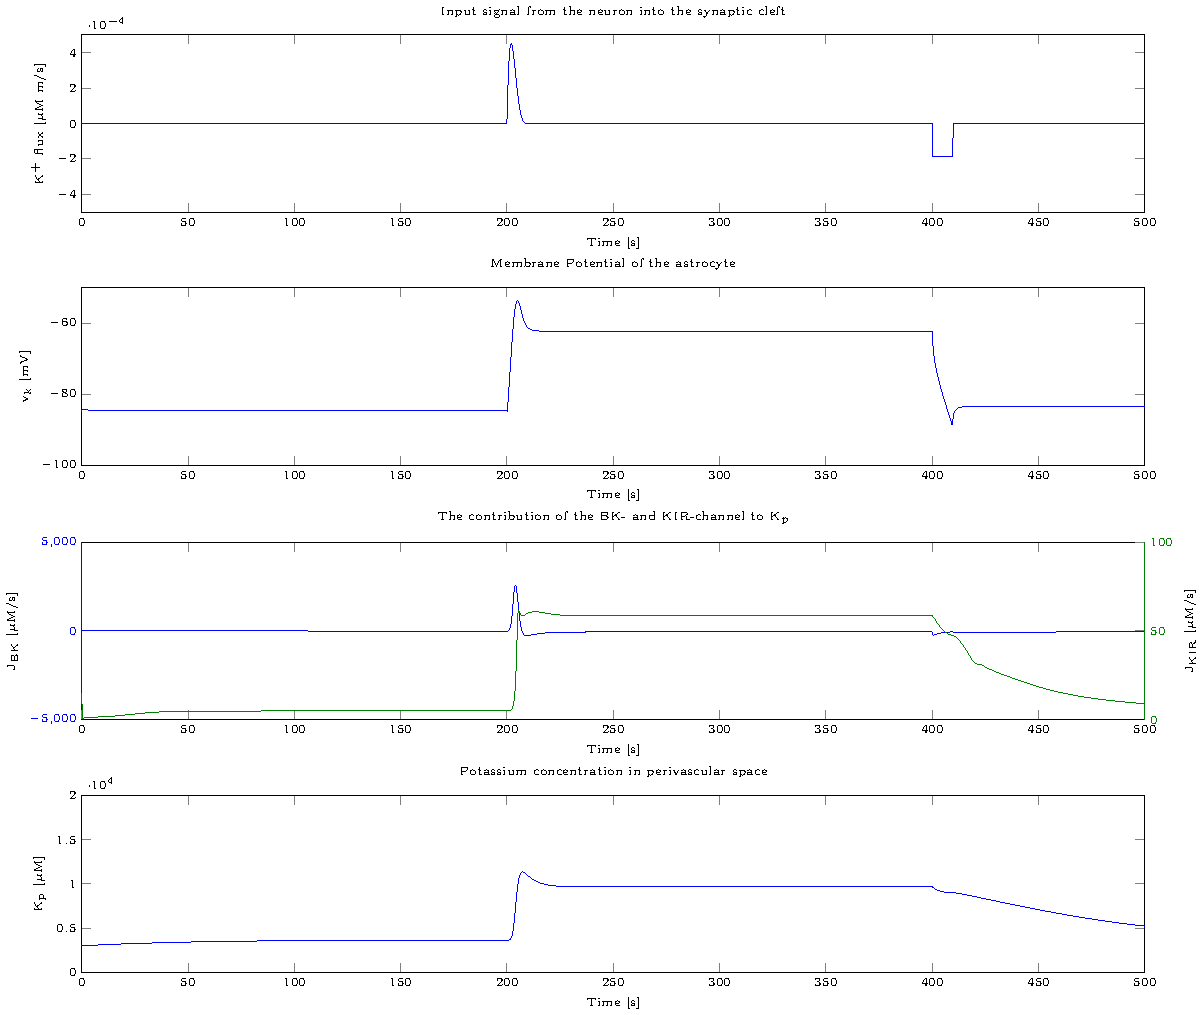
\includegraphics{figures/1_Input_signal.pdf}
			\caption{The input signal.}
			\label{fig:1IS}
		\end{figure}
		
		\begin{figure}[h!]
			\centering
			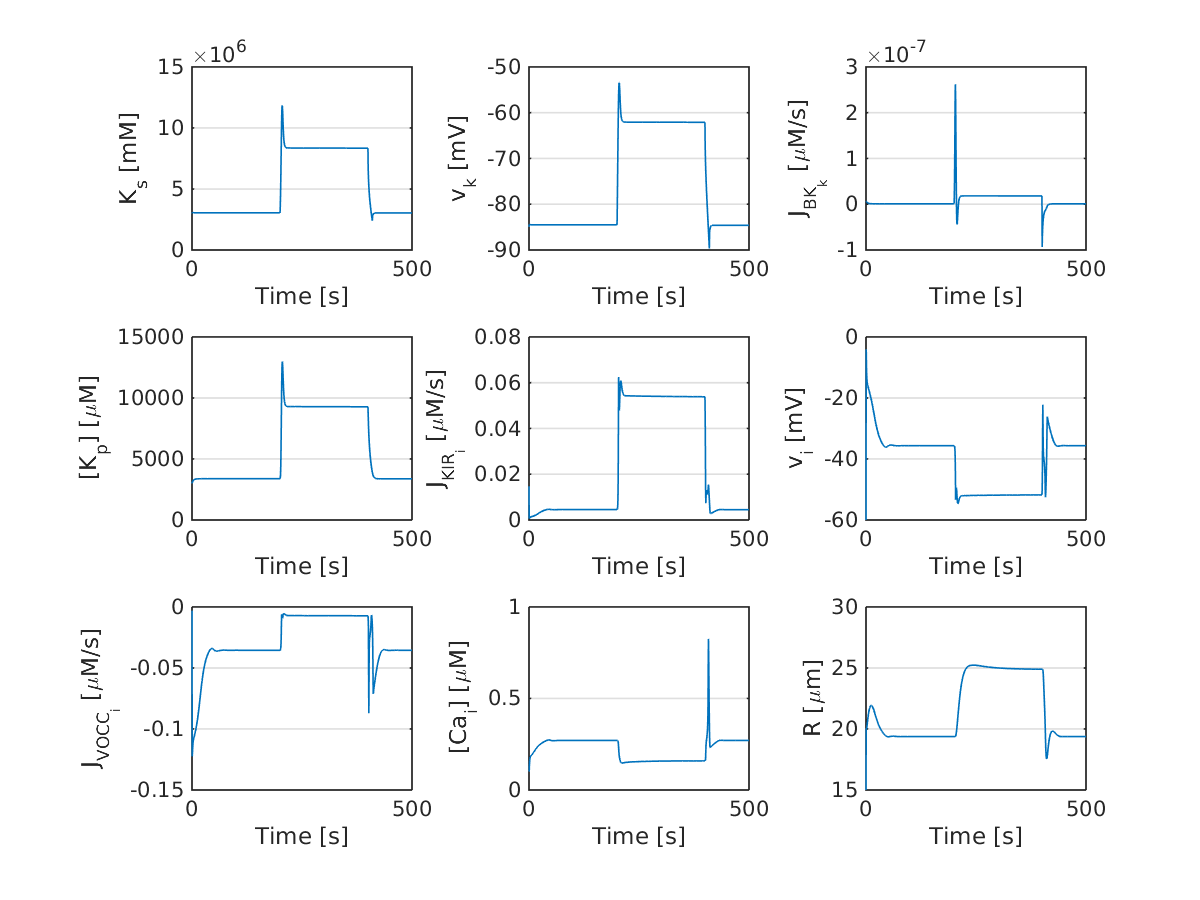
\includegraphics{new_figures/1 Neurovascular Coupling Overview.png}
			\caption{Neurovascular Coupling Overview.}
			\label{fig:1}
		\end{figure}		
		
		\begin{figure}[h!]
			\centering
			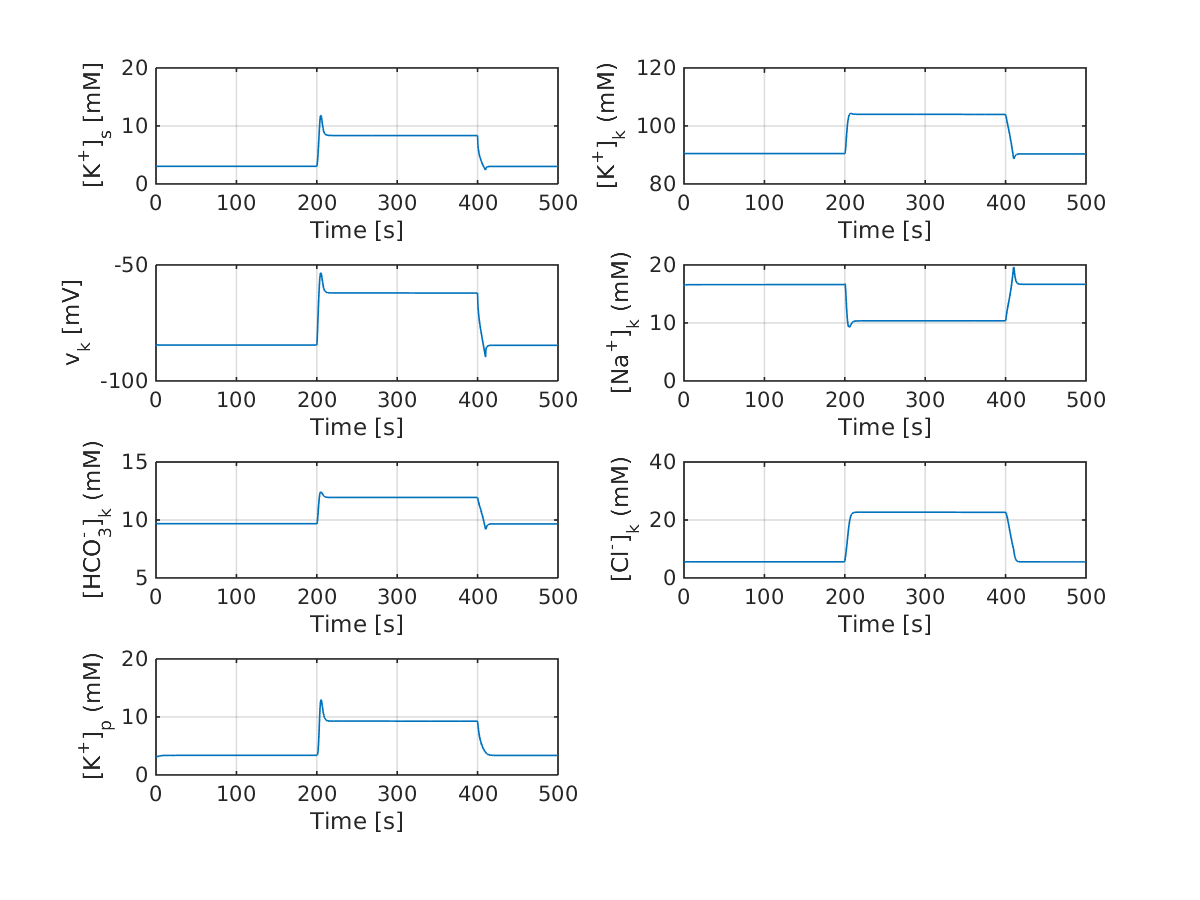
\includegraphics{new_figures/2 AC State Variables.png}
			\caption{AC State Variables.}
			\label{fig:2}
		\end{figure}
	
	
		\begin{figure}[h!]
			\centering
			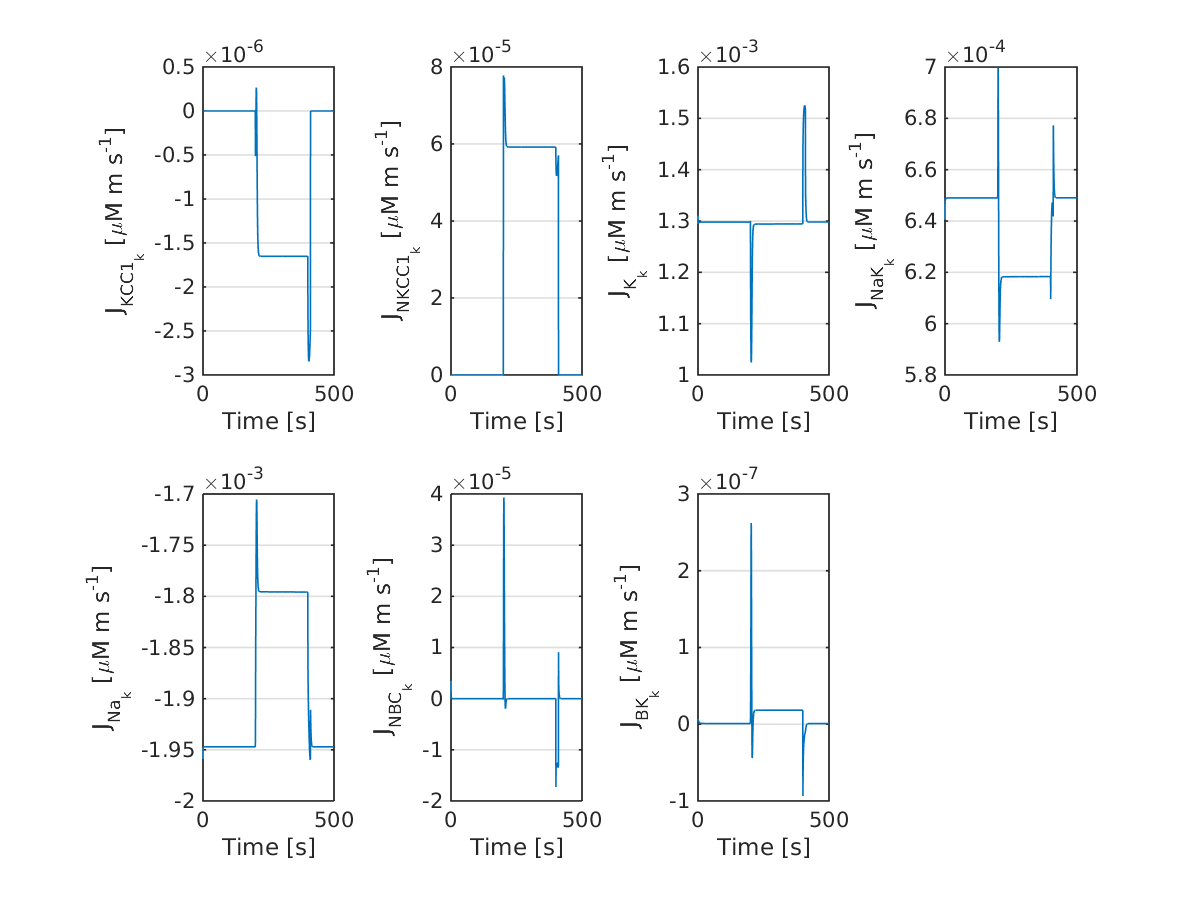
\includegraphics{new_figures/3 AC Fluxes.png}
			\caption{AC Fluxes.}
			\label{fig:3}
		\end{figure}
		
		
		\begin{figure}[h!]
			\centering
			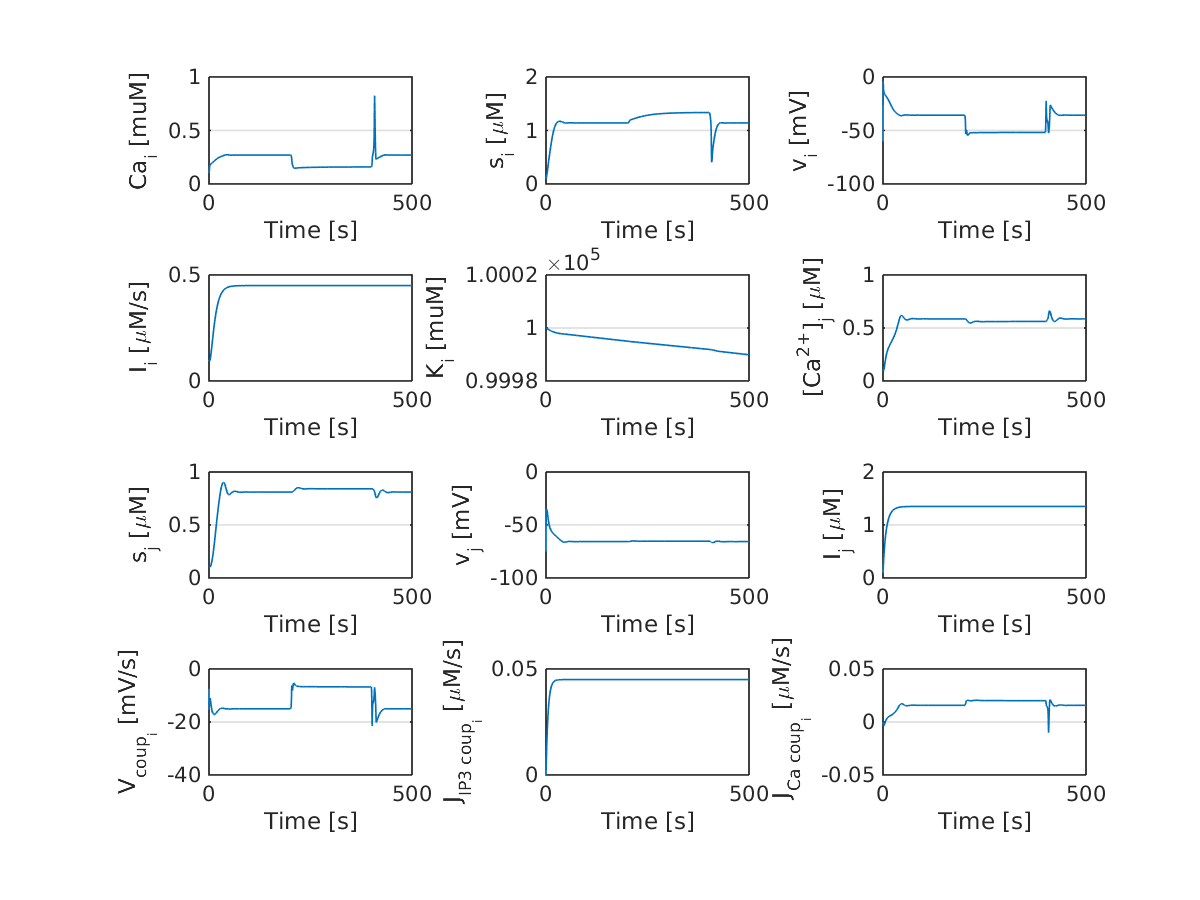
\includegraphics{new_figures/4 SMC EC State Variables and Coupling.png}
			\caption{SMC EC State Variables and Coupling.}
			\label{fig:4}
		\end{figure}
			
		\begin{figure}[h!]
			\centering
			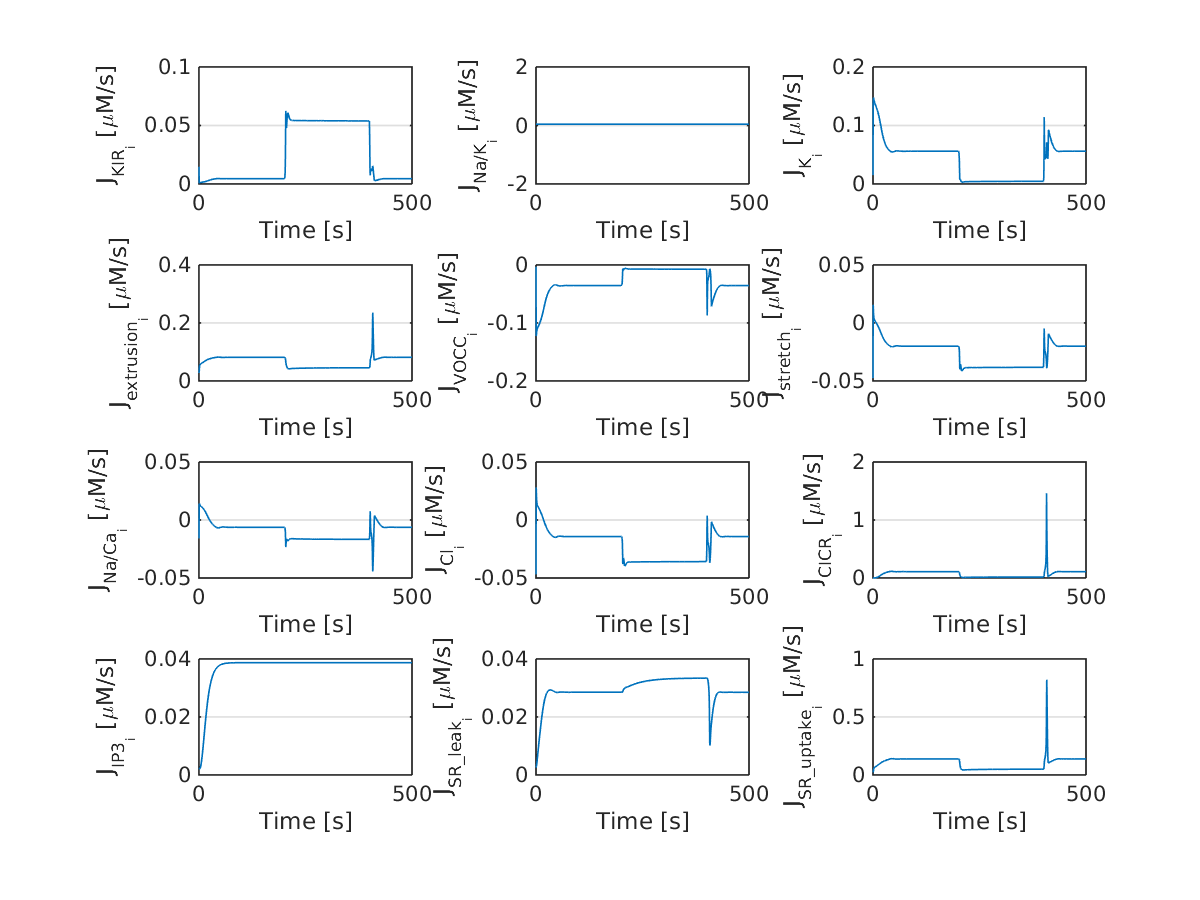
\includegraphics{new_figures/5 SMC Fluxes.png}
			\caption{SMC Fluxes.}
			\label{fig:5}
		\end{figure}
		
		\begin{figure}[h!]
			\centering
			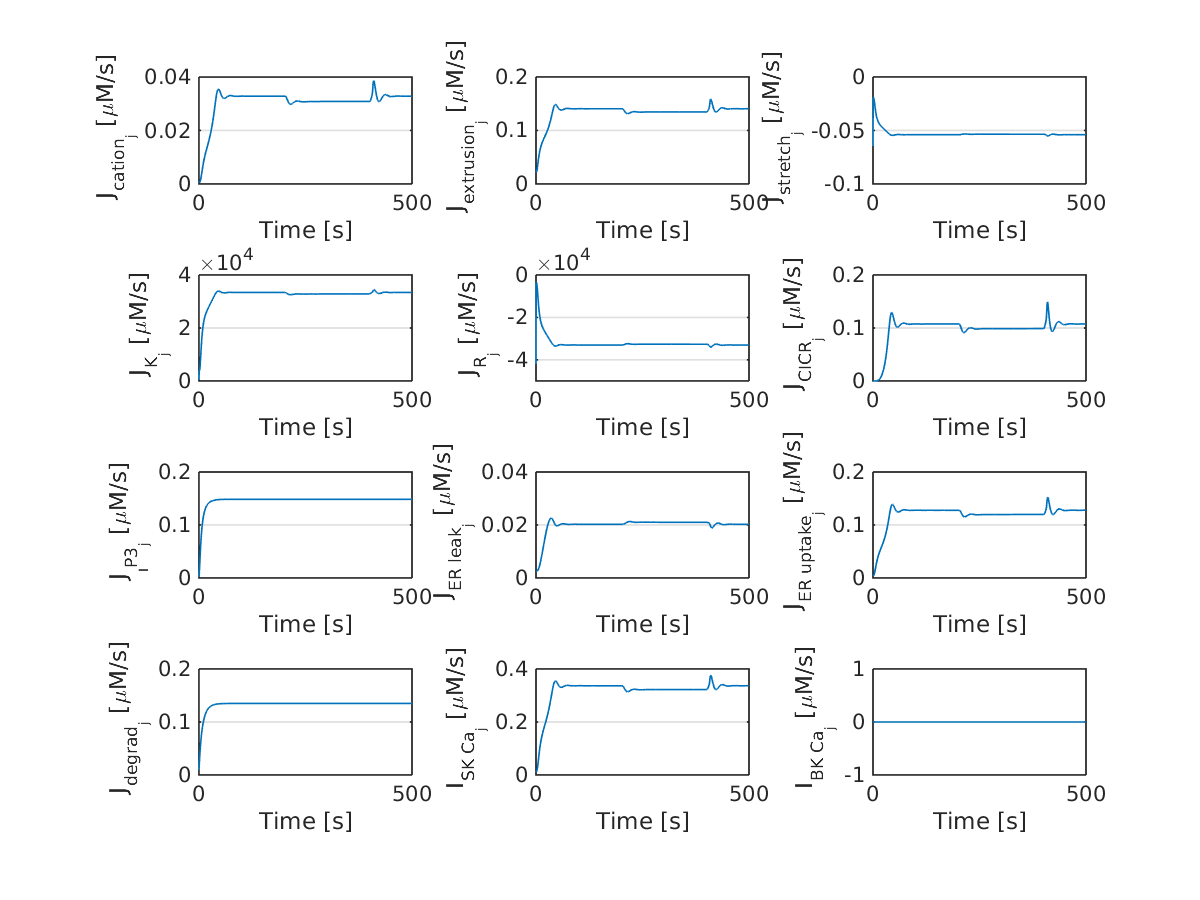
\includegraphics{new_figures/6 EC Fluxes.png}
			\caption{EC Fluxes.}
			\label{fig:6}
		\end{figure}
		
		\begin{figure}[h!]
			\centering
			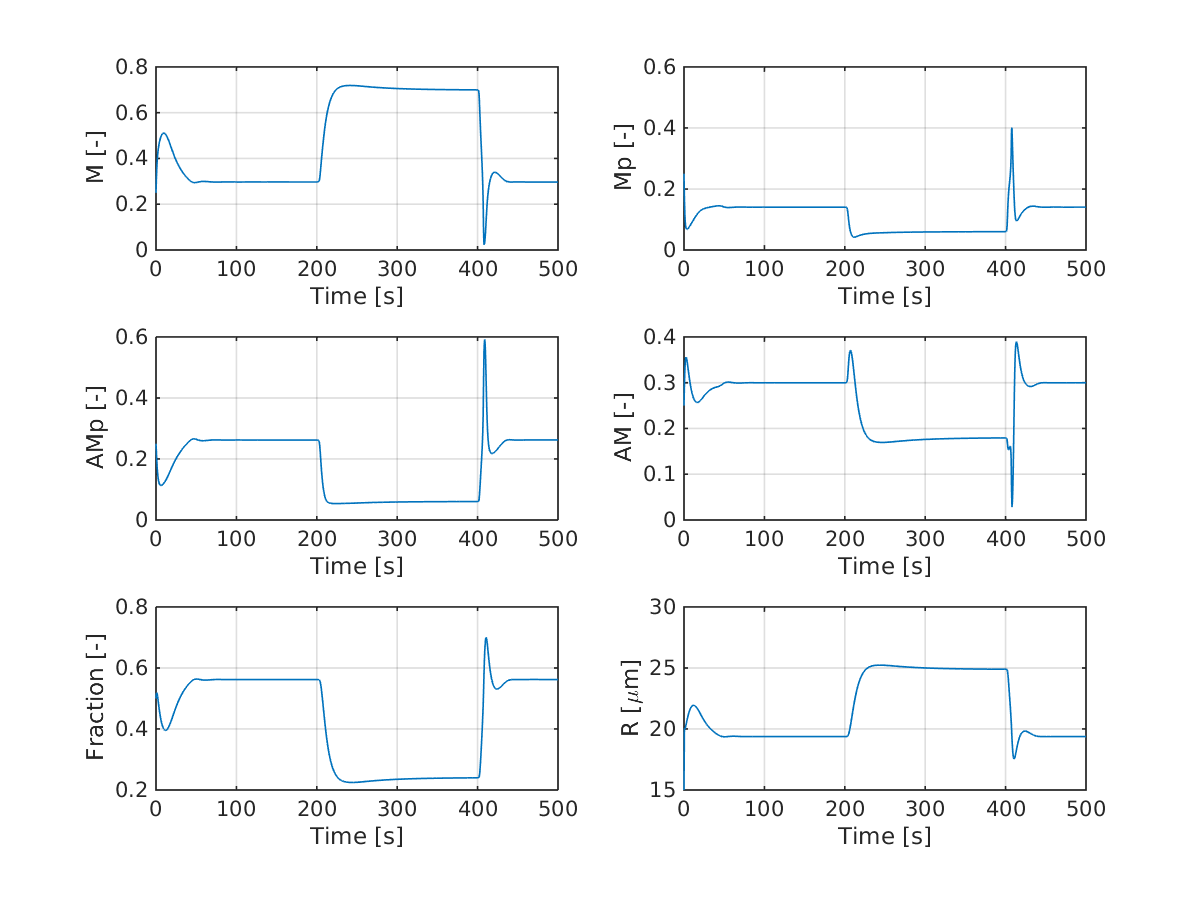
\includegraphics{new_figures/7 Contraction Model and Radius.png}
			\caption{Contraction Model and Radius.}
			\label{fig:7}
		\end{figure}
				
	\end{landscape}
	

\section{Equations}\label{sec:equations}
\todo[inline]{Some units need to be corrected in this documentation!}
\todo[inline]{add equations for NO in each section, add astrocyte calcium and trpv4 equations to that section, add glutamate signal}

\subsection{The Neuron and Astrocyte Model}

\subsubsection*{Input signals} \label{sec:InputSignal}

Neuronal \gls{K} input signal (dim.less):
\begin{equation}
f_{\text{K/Na}}(t) = 
	\begin{cases} 
		F_{\text{input}} \dfrac{(\alpha_n + \beta_n-1)!}{(\alpha_n-1)!(\beta_n-1)!} \left( \dfrac{1-(t-t_{0})}{\Delta t_2}\right) ^{\beta_n -1} \left( \dfrac{t-t_{0}}{\Delta t_2}\right) ^{\alpha_n -1}, & \text{for}\: t_{0} \leq t < t_{1} \\
		-F_{\text{input}}, & \text{for}\: t_{2} \leq t \leq t_{3} \\	
		0, & \text{otherwise}\\	
	\end{cases} 
\end{equation}

End of neuronal pulse (s):
\begin{equation}
	t_{1} = t_{0} + \Delta t
\end{equation}

Start of back-buffering (s):
\begin{equation}
	t_{2} = t_{0} + \Delta t_1
\end{equation}

End of back buffering (s):
\begin{equation}
	t_{3} = t_{1} + \Delta t_1
\end{equation}


\begin{table}[h!]
\centering
\begin{tabular}{ p{0.09\linewidth}  >{\footnotesize} p{0.5\linewidth}  >{\footnotesize} p{0.27\linewidth} >{\footnotesize} p{0.03\linewidth} }
\hline
$F_{\text{input}}$ 		& amplitude scaling factor 		& 2.5 		& ME\footnotemark[1]  \\ % on the basis of Filosa2008
$\alpha_n$ 				& beta distribution constant	& 2 		& ME  \\ % on the basis of Ostby2009
$\beta_n$ 				& beta distribution constant	& 5 		& ME  \\ % on the basis of Ostby2009
$t_{0}$ 				& start of neuronal activation	& 400 s 	& ME  \\
$\Delta t_1$ 			& length of neuronal activation & 200 s 	& ME  \\
$\Delta t_2$ 			& time-scaling factor			& 10 s		& \citep{Ostby2009}   \\
\hline
\end{tabular}
\end{table}
\footnote[1]{Model Estimation}

\subsubsection*{Scaling}
\gls{AC} volume-area ratio (in m):
\begin{equation} \label{eq:R_k}
	\begin{aligned}
	\dfrac{\mathrm{d}R_k}{\mathrm{d}t}= L_p([\Na]_k + [\K]_k + [\Cl]_k + [\HCO]_k - [\Na]_s - [\K]_s - [\Cl]_s - [\HCO]_s + \frac{X_k}{R_k})
	\end{aligned}
\end{equation}
%
\gls{SC} volume-surface ratio  (in m):
\begin{equation} \label{eq:R_tot}
R_s = R_{\text{tot}} - R_k  
\end{equation}

%Total volume-surface ratio (m):
%\begin{equation}
%	R_{\text{tot}} = \frac{V_{sc} + V_{k}}{A_k}
%\end{equation}

\begin{table}[h!]
\centering
\begin{tabular}{ p{0.09\linewidth}  >{\footnotesize} p{0.5\linewidth}  >{\footnotesize} p{0.27\linewidth} >{\footnotesize} p{0.03\linewidth} }
\hline
$L_p$ 			& total water permeability per unit area of the astrocyte  & 2.1\e{-9} \mperuMs &  \cite{Ostby2009}\footnotemark[2]  \\
$X_k$			& Number of negatively charged impermeable ions trapped within the astrocyte divided by the astrocyte membrane area								& 12.41$\times$10$^{-3}$ \uMm & \cite{Ostby2009}  \\
$R_{\text{tot}}$ 		& Total volume surface ratio AC + SC $ ((V_{sc} + V_{k})/A_k)  $ 		& 8.79$\times$10$^{-8}$ \m & \cite{Ostby2009}\footnotemark[2]  \\
%$V_{sc}$ 		& \gls{SC} volume   & 
$A_k$			& characteristic exchange surface area 	& 3.7\e{-9} m$^2$ & \citep{Ostby2009}\footnotemark[3]\\
\hline
\end{tabular}
\end{table}
\footnotetext[2]{corrected value/unit obtained from \texttt{CellML}}
\footnotetext[3]{corrected value/unit obtained from communication with author}
\subsubsection*{Conservation Equations}
\paragraph{Synaptic Cleft}~\\
%
\gls{K} concentration in the \gls{SC} (times the \gls{SC} volume-area ratio $R_s$; in \uMm):
\begin{equation} \label{eq:KEx}
\dfrac{\mathrm{d}N_{\text{K},s}}{\mathrm{d}t}= k_C f(t) -\dfrac{\mathrm{d}N_{\text{K},k}}{\mathrm{d}t} - J_{\text{BK},k}\,; \text{~~~} [\K]_s = \frac{N_{\text{K},s}}{R_s}
\end{equation}
%
\gls{Na} concentration in the \gls{SC}  (times the \gls{SC} volume-area ratio $R_s$; in \uMm):
\begin{equation} \label{eq:NaEx}
\dfrac{\mathrm{d}N_{\text{Na},s}}{\mathrm{d}t}= - k_C f(t) -\dfrac{\mathrm{d}N_{\text{Na},k}}{\mathrm{d}t}\,; \text{~~~} [\Na]_s = \frac{N_{\text{Na},s}}{R_s}
\end{equation}
%
\gls{HCO3} concentration in the SC  (times the \gls{SC} volume-area ratio $R_s$; in \uMm):
\begin{equation} \label{eq:HCOEx}
\dfrac{\mathrm{d}N_{\text{HCO}_3,s}}{\mathrm{d}t}=-\dfrac{\mathrm{d}N_{\text{HCO}_3,k}}{\mathrm{d}t}\,; \text{~~~} [\HCO]_s = \frac{N_{\text{HCO}_3,s}}{R_s}
\end{equation}
\begin{table}[h!]
\centering
\begin{tabular}{ p{0.09\linewidth}  >{\footnotesize} p{0.5\linewidth}  >{\footnotesize} p{0.27\linewidth} >{\footnotesize} p{0.03\linewidth} }
\hline
$ k_C $  & Input scaling parameter & 7.35$\times$10$^{-5}$ \muMps & \cite{Ostby2009} \\
\hline
\end{tabular}
\end{table}

\paragraph{Astrocyte}~\\
%
\gls{K} concentration in the AC  (times the AC volume-area ratio $R_k$; in \uMm):
\begin{equation} \label{eq:KInt}
\dfrac{\mathrm{d}N_{\text{K},k}}{\mathrm{d}t}=- J_{\text{K},k} + 2 J_{\text{NaK},k} + J_{NKCC1_{k}} +  J_{KCC1_{k}} - J_{\text{BK},k} \,; \text{~~~} [\K]_k = \frac{N_{\text{K},k}}{R_k}
\end{equation}
%
\gls{Na} concentration in the AC  (times the AC volume-area ratio $R_k$; in \uMm):
\begin{equation} \label{eq:NaInt}
\dfrac{\mathrm{d}N_{\text{Na},k}}{\mathrm{d}t}=-J_{\text{Na},k} - 3 J_{\text{NaK},k} + J_{NKCC1_{k}} +  J_{\text{NBC},k}\,; \text{~~~} [\Na]_k = \frac{N_{\text{Na},k}}{R_k}
\end{equation}
%
\gls{HCO3} concentration in the AC  (times the AC volume-area ratio $R_k$; in \uMm):
\begin{equation} \label{eq:HCOInt}
\dfrac{\mathrm{d}N_{\text{HCO}_3,k}}{\mathrm{d}t}= 2 J_{\text{NBC},k}\,; \text{~~~} [\HCO]_k = \frac{N_{\text{HCO}_3,k}}{R_k}
\end{equation}
%
\gls{Cl} concentration in the AC  (times the AC volume-area ratio $R_k$; in \uMm):
\begin{equation} \label{eq:ClInt}
\dfrac{\mathrm{d}N_{\text{Cl},k}}{\mathrm{d}t}= \dfrac{\mathrm{d}N_{\text{Na},k}}{\mathrm{d}t} + \dfrac{\mathrm{d}N_{\text{K},k}}{\mathrm{d}t} - \dfrac{\mathrm{d}N_{\text{HCO}_3,k}}{\mathrm{d}t}\,; \text{~~~} [\Cl]_k = \frac{N_{\text{Cl},k}}{R_k}
\end{equation}
%
Open probability of the BK channel (non-dim.):
\begin{equation} \label{eq:dwkdt}
\frac{\mathrm{d}w_{k}}{\mathrm{d}t} = \phi_{w} \left(w_{\infty}-w_{k} \right) 
\end{equation}
%
\paragraph{Perivascular Space}~\\
\gls{K} concentration in the PVS  (in \uM):
\begin{equation} \label{eq:K_p}
\dfrac{\mathrm{d}K_{p}}{\mathrm{d}t}= \frac{J_{\text{BK},k}}{R_k R_{pk}} + \frac{J_{\text{KIR},i}}{R_{ps}} - R_{\text{decay}}([\K]_p - [\K]_{p,\min});
\end{equation}
%
\begin{table}[h!]
\centering
\begin{tabular}{ p{0.09\linewidth}  >{\footnotesize} p{0.5\linewidth}  >{\footnotesize} p{0.27\linewidth} >{\footnotesize} p{0.03\linewidth} }
\hline
$ R_{pk} $  & Volume ratio of PVS to AC & 10$^{-3}$ [-] & \cite{Nagelhus1999} \\
$ R_{ps} $  & Volume ratio of PVS to SMC & 10$^{-3}$ [-] & \cite{Nagelhus1999} \\
$ R_{\text{decay}} $  & Decay rate & 0.05 s$^{-1}$ & M.E. \\
$ [\K]_{p,\min} $  & min \gls{K} concentration & 3 $\times$ 10$^{3}$ \textmu M & M.E. \\
\hline
\end{tabular}
\end{table}
\subsubsection*{Fluxes}\label{sec:EqNeAcflux}~\\ 
%
\gls{K} flux (times the AC volume-area ratio $R_k$; in \uMmps): 
\begin{equation} \label{eq:J_K}
J_{\text{K},k}=\frac{g_{K_{k}}}{F}(v_k - E_{\text{K},k})
\end{equation}
%
\gls{Na} flux (times the AC volume-area ratio $R_k$; in \uMmps):
\begin{equation} \label{eq:J_Na}
J_{\text{Na},k}=\frac{g_{Na_{k}}}{F}(v_k - E_{\text{Na},k})
\end{equation}
%
\gls{Na} and \gls{HCO3} flux through the NBC channel  (times the AC volume-area ratio $R_k$; in \uMmps): 
\begin{equation} \label{eq:J_NBC}
J_{\text{NBC},k}=\frac{g_{\text{NBC},k}}{F}\left(  v_k -E_{\text{NBC},k}  \right)
\end{equation}
%
\gls{Cl} and \gls{K} flux through the KCC1 channel  (times the AC volume-area ratio $R_k$; in \uMmps): 
\begin{equation} \label{eq:J_KCC1}
J_{\text{KCC1},k}=C_{input}\frac{g_{\text{KCC1},k}}{F}\frac{R_{\text{gas}}T}{F}ln \left(\frac{[\K]_s [\Cl]_s }{K_k [\Cl]_k}\right)
\end{equation}
%
\gls{Na}, \gls{K} and \gls{Cl} flux through the NKCC1 channel   (times the AC volume-area ratio $R_k$; in \uMmps): 
\begin{equation} \label{eq:J_NKCC1}
J_{\text{NKCC1},k}=C_{input}\frac{g_{\text{NKCC1},k}}{F}\frac{R_{\text{gas}}T}{F}ln \left(\frac{Na_s [\K]_s {[\Cl]_s}^2}{Na_k K_k {[\Cl]_k}^2}\right)
\end{equation}
%
Flux through the sodium potassium pump   (times the \gls{AC} volume-area ratio $R_k$; in \uMmps): 
\begin{equation} \label{eq:J_NaK_s}
J_{\text{NaK},k}=J_{\text{NaK,max}}\frac{{Na_k}^{1.5}}{{Na_k}^{1.5}+{K_{\text{Na},k}}^{1.5}}\frac{[\K]_s}{[\K]_s+K_{\text{K},s}}
\end{equation}
%
\gls{K} flux through the BK channel  (times the \gls{AC} volume-area ratio $R_k$; in \uMmps): 
\begin{equation} \label{eq:J_BK}
J_{\text{BK},k}=\frac{g_{\text{BK},k}}{F}w_k \left(v_k - E_{\text{BK},k} \right)
\end{equation}
%
%
%
\begin{table}[h!]
\centering
\begin{tabular}{ p{0.09\linewidth}  >{\footnotesize} p{0.5\linewidth}  >{\footnotesize} p{0.27\linewidth} >{\footnotesize} p{0.03\linewidth} }
\hline	
$F$ 			& Faraday's constant														& 9.649$\times$10$^4$ \Cmol 	& \\
$R_{\text{gas}}$ 			& Gas constant 															& 8.315 \JmolK		& \\
$T$ 	    	& Temperature 															& 300 \Kelvin		& \\
$g_{K_{k}}$ 	& Specific ion conductance of potassium 								& 40$\times$10$^3$ \perOhmm 		& \cite{Ostby2009}  \\
$g_{\text{Na},k}$ 		& Specific ion conductance of sodium 									& 1.314$\times$10$^3$  \perOhmm 	& \cite{Ostby2009}  \\
$g_{\text{NBC},k}$ 	& Specific ion conductance of the NBC cotransporter						& 7.57$\times$10$^2$ \perOhmm 	& \cite{Ostby2009}  \\
$g_{\text{KCC1},k}$ 	& Specific ion conductance of the KCC1 cotransporter					& 10 \perOhmm 	& \cite{Ostby2009}  \\
$g_{\text{NKCC1},k}$ 	& Specific ion conductance of the NKCC1 cotransporter	 				& 55.4 \perOhmm 	& \cite{Ostby2009}  \\
$J_{\text{NaK,max}}$ & Maximum flux through the NaKATPase pump						     	& 1.42$\times$10$^{-3}$ \uMms 	& \cite{Ostby2009}  \\
$G_{\text{BK},k}$ 		& Potassium conductance of the BK channel							& 4.3$\times$10$^3$   pS & \cite{GonzalezFernandez1994}  \\
%$A_{ef,k}$		& Membrane area														    & 3.7 $\times$ 10$^{-9}$ & \cite{GonzalezFernandez1994} \\
$C_{input}$  & Block function to switch the channel on and off &  0 ; 1 [-] 			&  \\
$K_{\text{Na},k}$  & Michaelis-Menten constant   &  10$^4$ \uM &   \\
$K_{\text{K},s}$  & Michaelis-Menten constant   &  1.5 $ \times $ 10$^3$ \uM &   \\
$C_{\text{unit}}$ & Unit converting factor   & 10$^{3}$ & M.E. \\
\hline
\end{tabular}
\end{table}


Specific ion conductance of the BK channel (\perOhmm):%  \cite{GonzalezFernandez1994}  
\begin{equation}
	g_{\text{BK},k} = \frac{G_{\text{BK},k} \times 10^{-12}}{A_{k}} = 1.16 \times 10^3 \text{ \perOhmm}
\end{equation}

\subsubsection*{Additional Equations}
\paragraph{Synaptic Cleft}~\\
%
\gls{Cl} concentration  (times the SC volume-area ratio $R_s$; in \uMm): 
\begin{equation} \label{eq:ClEx}
N_{\text{Cl},s}= N_{\text{Na},s}+N_{\text{K},s}-N_{ HCO_{3,s}}\,; \text{~~~} [\Cl]_s = \frac{N_{\text{Cl},s}}{R_s}
\end{equation}

\paragraph{Astrocyte}~\\
%
Membrane voltage of the \gls{AC} (V):
\begin{equation} \label{eq:v_k}
v_k = \frac{g_{\text{Na},k} E_{\text{Na},k} + g_{\text{K},k} E_{\text{K},k} + g_{\text{Cl},k}E_{\text{Cl},k}+g_{\text{NBC},k}E_{\text{NBC},k} + g_{\text{BK},k}w_kE_{\text{BK},k} -J_{\text{NaK},k}F C_{\text{unit}} } { g_{\text{Na},k}+g_{\text{K},k} + g_{\text{Cl},k} + g_{\text{NBC},k} + g_{\text{BK},k}w_k }
\end{equation}
%
Nernst potential for the potassium channel (in mV):
\begin{equation} \label{eq:E_K}
E_{\text{K},k}=\frac{R_{\text{gas}}T}{z_K F}ln\left( \frac{[\K]_s}{[\K]_k}\right) 
\end{equation}
%
Nernst potential for the sodium channel (in mV):
\begin{equation} \label{eq:E_Na}
E_{\text{Na},k}=\frac{R_{\text{gas}}T}{z_{\text{Na}} F}ln\left( \frac{Na_s}{Na_k}\right) 
\end{equation}
%
Nernst potential for the chloride channel (in mV):
\begin{equation} \label{eq:E_Cl}
E_{\text{Cl},k} = \frac{R_{\text{gas}}T}{z_{\text{Cl}} F}ln\left( \frac{[\Cl]_s}{[\Cl]_k}\right) 
\end{equation}
%
Nernst potential for the NBC channel (in mV):
\begin{equation} \label{eq:E_NBC}
E_{\text{NBC},k} = \frac{R_{\text{gas}}T}{z_{NBC} F}ln\left( \frac{Na_s {HCO_{3,s}}^2}{Na_k {HCO_{3,k}}^2}\right) 
\end{equation}
Nernst potential for the BK channel (in mV):
\begin{equation} \label{eq:E_BK}
E_{\text{BK},k} = \frac{R_{\text{gas}} T}{z_K F}\ln\left( \frac{[\K]_p}{[\K]_k}\right) 
\end{equation}
%
Equilibrium state BK-channel (-):
\begin{equation} \label{eq:winf}
w_{\infty} = 0.5 \left(1+\tanh\left(\frac{v_{k}+v_{6} }{v_{4}} \right)  \right) 
\end{equation}
%
Time constant associated with the opening of BK channels	 (in \pers):
\begin{equation} \label{eq:phin}
\phi_{w} = \psi_{w}\cosh\left( \frac{v_{k}+v_{6}}{2v_{4}}\right) 
\end{equation}

\begin{table}[h!]
\centering
\begin{tabular}{ p{0.09\linewidth}  >{\footnotesize} p{0.6\linewidth}  >{\footnotesize} p{0.17\linewidth} >{\footnotesize} p{0.03\linewidth} }
\hline
$g_{\text{Cl},k}$ 		& Specific ion conductance of chloride 									& 0.879 \perOhmm & \cite{Ostby2009}  \\
$z_K$			& Valence of a potassium ion										& 1   & \\ 
$z_{\text{Na}}$			& Valence of a sodium ion											& 1   & \\ 
$z_{\text{Cl}}$			& Valence of a chloride ion											& -1  & \\ 
$z_{NBC}$ 		& Effective valence of the NBC cotransporter complex 				& -1 & \\
$v_{6}$			& Voltage associated with the opening of half the population		& 22 mV or V???  & \cite{GonzalezFernandez1994}  \\
$v_{4}$			& A measure of the spread of the distribution of the open probability of the BK channel	& 14.5 mV or V???  &  \cite{GonzalezFernandez1994}  
\\
$ \psi_{w}$    	& A characteristic time for the open probability of the BK channel		& 2.664 \pers & \cite{GonzalezFernandez1994} \\
\hline
\end{tabular}
\end{table}

\subsection{The Smooth Muscle Cell and Endothelial Cell Model}\label{sec:EqSMCEC}

\subsubsection*{Conservation Equations}
\paragraph{Smooth muscle cell}~\\
%
Cytosolic [\gls{Ca}] in the \gls{SMC} (in \uM):
\begin{equation}\label{eq:ci}
\begin{split}
\dfrac{\mathrm{d}\CaConsc}{\mathrm{d}t} = J_{\text{IP}_3,i} - J_{\text{upt},i} + J_{\text{CICR}_i} - J_{\text{extr},i} +  J_{\text{leak},i}\dots \\
 - J_{\text{VOCC},i} + J_{\text{Na/Ca},i}  + 0.1J_{\text{stretch},i} + J_{Ca^{2+}-coupling_{i}}^{SMC-EC}
\end{split} 
\end{equation}
%
[Ca$^{2+}$] in the \gls{SR} of the \gls{SMC} (in \uM):
\begin{equation} \label{eq:si}
\dfrac{\mathrm{d}\CaConse}{\mathrm{d}t} =  J_{\text{upt},i} - J_{\text{CICR}_i} - J_{\text{leak},i}
\end{equation}
%
Membrane potential of the \gls{SMC} (in \mV):
\begin{equation} \label{eq:vi}
\begin{split}
\dfrac{\mathrm{d}v_{i}}{\mathrm{d}t} = \gamma_{i}( -J_{\text{Na/K},i} - J_{\text{Cl},i} - 2J_{\text{VOCC},i}- J_{\text{Na/Ca},i} - J_{\text{K},i} \dots \\
- J_{\text{stretch},i} - J_{\text{KIR},i} ) +V^{SMC-EC}_{coupling_{i}}
\end{split}
\end{equation}
%
Open state probability of calcium-activated potassium channels (dim.less):
\begin{equation} \label{eq:dwidt}
\dfrac{\mathrm{d}w_{i}}{\mathrm{d}t} =  \lambda_{i} \left( K_{act_{i}} - w_{i} \right)
\end{equation}
%
\gls{IP3} concentration om the \gls{SMC} (in \uM):
\begin{equation} \label{eq:dIidt}
\dfrac{\mathrm{d}\IP _{i}}{\mathrm{d}t} = J^{SMC-EC}_{IP_{3}-coupling_{i}} - J_{\text{degr},i}
\end{equation}
%
\gls{K} concentration in the \gls{SMC} (in \uM):
\begin{equation} \label{eq:dkidt}
\dfrac{\mathrm{d} [\K]_i}{\mathrm{d}t}  = J_{\text{Na/K},i}  - J_{\text{KIR},i} - J_{\text{K},i}
\end{equation}

\begin{table}[h!]
\centering
\begin{tabular}{ p{0.09\linewidth}  >{\footnotesize} p{0.5\linewidth}  >{\footnotesize} p{0.27\linewidth} >{\footnotesize} p{0.03\linewidth} }
\hline
$\gamma_{i}$				& Change in membrane potential by a scaling factor					& 1970 \mVpuM	& \cite{Koenigsberger2006} \\
$\lambda_{i} $				& Rate constant for opening											& 45.0 \pers 	& \cite{Koenigsberger2006} \\
%$\CaConsc$      		& Cytololic [Ca$^{2+}$] in the SMC    								& var. \uM		& - \\
\hline
\end{tabular}
\label{tab:dcidt}
\end{table}

\paragraph{Endothelial cell}~\\
%
Cytosolic \gls{Ca} concentration in the \gls{EC} (in \uM):
\begin{equation} \label{eq:cj}
\begin{split}
\dfrac{\mathrm{d}\CaConec}{\mathrm{d}t} = J_{\text{IP}_3,j} - J_{\text{upt},j} + J_{CICR_{j}} - J_{\text{extr},j}\dots \\
 + J_{\text{leak},j} + J_{cation_{j}} + J_{0_{j}} + J_{\text{stretch},j} - J_{Ca^{2+}-coupling_{j}}^{SMC-EC}
\end{split}
\end{equation}
%
\gls{Ca} concentration in the \gls{ER} in the \gls{EC} (in \uM): %copied from SMC
\begin{equation} \label{eq:sj}
\dfrac{\mathrm{d}\CaConee}{\mathrm{d}t} =  J_{\text{upt},j} - J_{CICR_{j}} - J_{\text{leak},j}
\end{equation}
%
Membrane potential of the \gls{EC} (in \mV):
\begin{equation} \label{eq:dvjdt}
\dfrac{\mathrm{d}v_{j}}{\mathrm{d}t} =-\frac{1}{C_{m_{j}}} ( J_{K_{j}}+J_{R_{j}}) + V^{SMC-EC}_{coupling_{j}}
\end{equation}
%
\gls{IP3} concentration of the \gls{EC} (in \uM):
\begin{equation} \label{eq:dIjdt}
\dfrac{\mathrm{d}\IP_{j}}{\mathrm{d}t} =  J_{\text{EC,IP}_3}- J_{\text{degr},j}  - J^{SMC-EC}_{IP_{3}-coupling_{j}}
\end{equation}

\begin{table}[h!]
\centering
\begin{tabular}{ p{0.09\linewidth}  >{\footnotesize} p{0.5\linewidth}  >{\footnotesize} p{0.27\linewidth} >{\footnotesize} p{0.03\linewidth} }
\hline
 $C_{m_{j}}$				& Membrane capacitance												& 25.8  \pF		& \cite{Koenigsberger2006} \\
 $ J_{PLC} $  & PLC / \gls{IP3} production rate & 0.18 or 0.4 \uMps & \cite{Koenigsberger2006}  \\
 $J_{0_{j}}$ & Constant Ca2+ leak term (influx) & 0.029 \uMps & \cite{Koenigsberger2006} \\ 
\hline
\end{tabular}
\label{tab:JSRuptakei}
\end{table}
%\\

\subsubsection*{Fluxes}
%
\paragraph{Smooth muscle cell}~\\
%
Release of calcium from IP$_{3}$ sensitive stores in the SMC (in \uMps):
\begin{equation} \label{eq:IP3i}
J_{\text{IP}_3,i} = F_{i}\frac{\IP_{i}^{2}}{K_{ri}^{2}+\IP_{i}^{2}}
\end{equation}
%
\begin{table}[h!]
\centering
\begin{tabular}{ p{0.09\linewidth}  >{\footnotesize} p{0.5\linewidth}  >{\footnotesize} p{0.27\linewidth} >{\footnotesize} p{0.03\linewidth} }
\hline
 $F_{i}$      			& Maximal rate of activation-dependent calcium influx			& 0.23 \uMps				& \cite{Koenigsberger2006} \\
$K_{ri}$				& Half-saturation constant for agonist-dependent calcium entry	& 1 \uM					& \cite{Koenigsberger2006} \\
\hline
\end{tabular}
\label{tab:IP3i}
\end{table}
\\
%
Uptake of calcium into the sarcoplasmic reticulum (in \uMs):
\begin{equation} \label{eq:JSRuptakei}
J_{\text{upt},i} = B_{i}\frac{\CaConsc^{2}}{c_{bi}^{2}+\CaConsc^{2}}
\end{equation}
%
\begin{table}[h!]
\centering
\begin{tabular}{ p{0.09\linewidth}  >{\footnotesize} p{0.5\linewidth}  >{\footnotesize} p{0.27\linewidth} >{\footnotesize} p{0.03\linewidth} }
\hline
$B_{i}$      			& SR uptake rate constant							& 2.025 \uMs				& \cite{Koenigsberger2006} \\
$c_{bi}$				& Half-point of the SR ATPase activation sigmoidal 	& 1.0 \uM					& \cite{Koenigsberger2006} \\
\hline
\end{tabular}
\label{tab:JSRuptakei}
\end{table}
\\
%
Calcium-induced calcium release (CICR; in \uMs):
\begin{equation} \label{eq:JCICRi}
J_{\text{CICR}_i} = C_{i}\frac{\CaConse^{2}}{s_{ci}^{2}+\CaConse^{2}}    \frac{\CaConsc^{4}}{c_{ci}^{4}+\CaConsc^{4}}
\end{equation}
%
\begin{table}[h!]
\centering
\begin{tabular}{ p{0.09\linewidth}  >{\footnotesize} p{0.5\linewidth}  >{\footnotesize} p{0.27\linewidth} >{\footnotesize} p{0.03\linewidth} }
\hline
$C_{i}$      			& CICR rate constant									& 55 \uMs		& \cite{Koenigsberger2006} \\
$s_{ci}$				& Half-point of the CICR Ca$^{2+}$ efflux sigmoidal			& 2.0 \uM		& \cite{Koenigsberger2006} \\
$c_{ci}$				& Half-point of the CICR activation sigmoidal			& 0.9 \uM		& \cite{Koenigsberger2006} \\
\hline
\end{tabular}
\label{tab:JCICRi}
\end{table}
\\
%
Calcium extrusion by Ca$^{2+}$-ATPase pumps (in \uMs):
\begin{equation} \label{eq:Jextrusioni}
J_{\text{extr},i} = D_{i}\CaConsc   \left( 1+ \frac{v_{i}-v_{d}}{R_{di}}\right)
\end{equation}
%
\begin{table}[h!]
\centering
\begin{tabular}{ p{0.09\linewidth}  >{\footnotesize} p{0.5\linewidth}  >{\footnotesize} p{0.27\linewidth} >{\footnotesize} p{0.03\linewidth} }
\hline
$D_{i}$      			& Rate constant for Ca$^{2+}$ extrusion by the ATPase pump		 & 0.24	\pers			& \cite{Koenigsberger2006} \\
$v_{d}$					& Intercept of voltage dependence of extrusion ATPase			 & -100.0 \mV			& \cite{Koenigsberger2006} \\
$R_{di}$				& Slope of voltage dependence of extrusion ATPase.				 & 250.0 \mV			& \cite{Koenigsberger2006} \\
\hline
\end{tabular}
\label{tab:Jextrusioni}
\end{table}
\\
%
Leak current from the SR (in \uMs):
\begin{equation} \label{eq:JSRleaki}
J_{\text{leak},i} = L_{i}\CaConse
\end{equation}
\begin{table}[h!]
\centering
\begin{tabular}{ p{0.09\linewidth}  >{\footnotesize} p{0.5\linewidth}  >{\footnotesize} p{0.27\linewidth} >{\footnotesize} p{0.03\linewidth} }
\hline
$L_{i}$      			& Leak from SR rate constant						 & 0.025 \pers				& \cite{Koenigsberger2006} \\
\hline
\end{tabular}
\label{tab:Jleaki}
\end{table}
\\

Calcium influx through VOCCs (in \uMs): 
\begin{equation} \label{eq:JVOCCi}
J_{\text{VOCC},i} = G_{\text{Ca},i} \frac{v_{i}-v_{\text{Ca}_1,i}}     {1+ \exp(-\left[ \left(  v_{i}-v_{\text{Ca}_2,i}\right) /R_{\text{Ca},i}      \right] )}
\end{equation}
\begin{table}[h!]
\centering
\begin{tabular}{ p{0.09\linewidth}  >{\footnotesize} p{0.5\linewidth}  >{\footnotesize} p{0.27\linewidth} >{\footnotesize} p{0.03\linewidth} }
\hline
$G_{\text{Ca},i}$      	& Whole-cell conductance for VOCCs	 					& 1.29$\times$10$^{-3}$  \uMpmVs					& \cite{Koenigsberger2006} \\
$v_{\text{Ca}_1,i}$   & Reversal potential for VOCCs	 						& 100.0 \mV							& \cite{Koenigsberger2006} \\
$v_{\text{Ca}_2,i}$  	& Half-point of the VOCC activation sigmoidal		 	& -24.0 \mV							& \cite{Koenigsberger2006} \\
$R_{\text{Ca},i}$      	& Maximum slope of the VOCC	activation sigmoidal		& 8.5 \mV							& \cite{Koenigsberger2006} \\
\hline
\end{tabular}
\label{tab:JVOCCi}
\end{table}
\newpage
Flux of calcium exchanging with sodium in the Na$^{+}$Ca$^{2+}$ exchange (in \uMs): 
\begin{equation} \label{eq:JNaCai}
J_{\text{Na/Ca},i} = G_{\text{Na/Ca},i} \frac{\CaConsc}     {\CaConsc + c_{\text{Na/Ca},i}} \left( v_{i}-v_{\text{Na/Ca},i} \right)
\end{equation}
%
\begin{table}[h!]
\centering
\begin{tabular}{ p{0.09\linewidth}  >{\footnotesize} p{0.5\linewidth}  >{\footnotesize} p{0.27\linewidth} >{\footnotesize} p{0.03\linewidth} }
\hline
$G_{\text{Na/Ca},i}$   	& Whole-cell conductance for Na$^{+}$/Ca$^{2+}$ exchange			 		 & 3.16$\times$10$^{-3}$ \uMpmVs	& \cite{Koenigsberger2006} \\
$c_{\text{Na/Ca},i}$   	& Half-point for activation of Na$^{+}$/Ca$^{2+}$ exchange by Ca$^{2+}$		 & 0.5 \uM			& \cite{Koenigsberger2006} \\
$v_{\text{Na/Ca},i}$   	& Reversal potential for the Na$^{+}$/Ca$^{2+}$ exchanger					 & -30.0 \mV		& \cite{Koenigsberger2006} \\
\hline
\end{tabular}
\label{tab:JNaCai}
\end{table}
\\
%
Calcium flux through the stretch-activated channels in the SMC (in \uMs): 
\begin{equation} \label{eq:Jstretchi}
\begin{split}
J_{\text{stretch},i}= \frac{G_{\text{stretch}}}{1+ \exp\left(-\alpha_{\text{stretch}}  \left(  \frac{\Delta pR}{h} -\sigma_{0}   \right) \right)}  \left(  v_{i}-E_{\text{SAC}}   \right) 
\end{split}
\end{equation}
%
\begin{table}[h!]
\centering
\begin{tabular}{ p{0.09\linewidth}  >{\footnotesize} p{0.5\linewidth}  >{\footnotesize} p{0.27\linewidth} >{\footnotesize} p{0.03\linewidth} }
\hline
$G_{\text{stretch}}$      		& Whole cell conductance for SACs						& 6.1$\times$10$^{-3}$ \uMpmVs	&\cite{Koenigsberger2006} \\
$\alpha_{\text{stretch}}$      & Slope of stress dependence of the SAC activation sigmoidal	& 7.4$\times$10$^{-3}$ \pmmHg	&\cite{Koenigsberger2006} \\
$ \Delta p $			& Pressure difference										& 30 \mmHg			& ME \\
$\sigma_{0}$      		& Half-point of the SAC activation sigmoidal				& 500 \mmHg			&\cite{Koenigsberger2006} \\
$E_{\text{SAC}}$      			& Reversal potential for SACs							& -18 \mV			&\cite{Koenigsberger2006} \\
\hline
\end{tabular}
\label{tab:Jstretchi}
\end{table}
\\
%
Flux through the sodium potassium pump (in \uMs): 
\begin{equation} \label{eq:J_NaK_i}
J_{\text{Na/K},i}= F_{\text{Na/K},i}
\end{equation}
%
\begin{table}[h!]
\centering
\begin{tabular}{ p{0.09\linewidth}  >{\footnotesize} p{0.5\linewidth}  >{\footnotesize} p{0.27\linewidth} >{\footnotesize} p{0.03\linewidth} }
\hline
$F_{\text{Na/K},i}$      			& Rate of the potassium influx by the sodium potassium pump 		& 4.32$\times$10$^{-2}$ \uMps 	&\cite{Koenigsberger2006} \\
\hline
\end{tabular}
\label{tab:JCli}
\end{table}
\\
Chloride flux through the chloride channel (in \uMs):
\begin{equation} \label{eq:JCli}
J_{\text{Cl},i} = G_{\text{Cl},i} \left(  v_{i} - v_{\text{Cl},i}  \right) 
\end{equation}
%
\begin{table}[h!]
\centering
\begin{tabular}{ p{0.09\linewidth}  >{\footnotesize} p{0.5\linewidth}  >{\footnotesize} p{0.27\linewidth} >{\footnotesize} p{0.03\linewidth} }
\hline
$G_{\text{Cl},i}$      			& Whole-cell conductance for Cl$^{-}$ current		& 1.34$\times$10$^{-3}$ \uMpmVs	&\cite{Koenigsberger2006} \\
$v_{\text{Cl},i}$      			& Reversal potential for Cl$^{-}$ channels.			& -25.0 \mV			&\cite{Koenigsberger2006} \\
\hline
\end{tabular}
\label{tab:JCli}
\end{table}
\\
%
Potassium flux through potassium channel (in \uMs):
\begin{equation} \label{eq:JKi}
J_{\text{K},i}= G_{\text{K},i} w_{i} \left(  v_{i} - v_{K_i}  \right) 
\end{equation}
%
\begin{table}[h!]
\centering
\begin{tabular}{ p{0.09\linewidth}  >{\footnotesize} p{0.5\linewidth}  >{\footnotesize} p{0.27\linewidth} >{\footnotesize} p{0.03\linewidth} }
\hline
$G_{\text{K},i}$      			& Whole-cell conductance for K$^{+}$ efflux.			& 4.46$\times$10$^{-3}$ \uMpmVs	&\cite{Koenigsberger2006} \\
$v_{K_i}$      			& Nernst potential										& -94 \mV	&\cite{Koenigsberger2006} \\
\hline
\end{tabular}
\label{tab:JKi}
\end{table}
\\
Flux through KIR channels in the SMC (in \uMs): 
\begin{equation} \label{eq:JKIRi}
J_{\text{KIR},i} =  \frac{F_{\text{KIR},i} g_{\text{KIR},i}}{\gamma_{i}}( v_{i} - v_{\text{KIR},i})
\end{equation}
\begin{table}[h!]
\centering
\begin{tabular}{ p{0.09\linewidth}  >{\footnotesize} p{0.5\linewidth}  >{\footnotesize} p{0.27\linewidth} >{\footnotesize} p{0.03\linewidth} }
\hline
$ F_{\text{KIR},i} $ & Scaling factor of potassium efflux through the KIR channel & 750 mV~\textmu M$^{-1}$ & \cite{GonzalezFernandez1994} \\
\hline
\end{tabular}
\label{tab:JCli}
\end{table}
\\
IP$_{3}$ degradation (in \uMs): 
\begin{equation} \label{eq:Jdegradi}
J_{\text{degr},i}= k_{\text{d},i}\IP_i
\end{equation}
\begin{table}[h!]
\centering
\begin{tabular}{ p{0.09\linewidth}  >{\footnotesize} p{0.5\linewidth}  >{\footnotesize} p{0.27\linewidth} >{\footnotesize} p{0.03\linewidth} }
\hline
$k_{\text{d},i}$      			& Rate constant of IP$_{3}$ degradation	& 0.1 \pers	&\cite{Koenigsberger2006} \\
\hline
\end{tabular}
\label{tab:Jdegradi}
\end{table}
\paragraph{Endothelial cell}~\\
\\
%
Release of calcium from IP$_{3}$-sensitive stores in the EC (in \uMps):
\begin{equation} \label{eq:JIP3j}
J_{\text{IP}_3,j} = F_{j}\frac{\IP_{j}^{2}}{K_{rj}^{2}+\IP_{j}^{2}}
\end{equation}
\begin{table}[h!]
\centering
\begin{tabular}{ p{0.09\linewidth}  >{\footnotesize} p{0.5\linewidth}  >{\footnotesize} p{0.27\linewidth} >{\footnotesize} p{0.03\linewidth} }
\hline
 $F_{j}$      			& Maximal rate of activation-dependent calcium influx			& 0.23 \uMps				& \cite{Koenigsberger2006} \\
$K_{rj}$				& Half-saturation constant for agonist-dependent calcium entry	& 1 \uM					& \cite{Koenigsberger2006} \\
\hline
\end{tabular}
\label{tab:IP3j}
\end{table}
\\
%
Uptake of calcium into the endoplasmic reticulum (in \uMs):
\begin{equation} \label{eq:JERuptakej}
J_{\text{upt},j} = B_{j}\frac{\CaConec^{2}}{c_{bj}^{2}+\CaConec^{2}}
\end{equation}
%
\begin{table}[h!]
\centering
\begin{tabular}{ p{0.09\linewidth}  >{\footnotesize} p{0.5\linewidth}  >{\footnotesize} p{0.27\linewidth} >{\footnotesize} p{0.03\linewidth} }
\hline
$B_{j}$      			& ER uptake rate constant							& 0.5 \uMs				& \cite{Koenigsberger2006} \\
$c_{bj}$				& Half-point of the SR ATPase activation sigmoidal 	& 1.0 \uM					& \cite{Koenigsberger2006} \\
\hline
\end{tabular}
\label{tab:JERuptakej}
\end{table}
\\
%
Calcium-induced calcium release (CICR; in \uMs):
\begin{equation} \label{eq:JCICRJ}
J_{CICR_{j}} = C_{j}\frac{\CaConee^{2}}{s_{cj}^{2}+\CaConee^{2}}    \frac{\CaConec^{4}}{c_{cj}^{4}+\CaConec^{4}}
\end{equation}
%
\begin{table}[h!]
\centering
\begin{tabular}{ p{0.09\linewidth}  >{\footnotesize} p{0.5\linewidth}  >{\footnotesize} p{0.27\linewidth} >{\footnotesize} p{0.03\linewidth} }
\hline
$C_{j}$      			& CICR rate constant									& 5 \uMs		& \cite{Koenigsberger2006} \\
$s_{cj}$				& Half-point of the CICR Ca$^{2+}$ efflux sigmoidal			& 2.0 \uM		& \cite{Koenigsberger2006} \\
$c_{cj}$				& Half-point of the CICR activation sigmoidal			& 0.9 \uM		& \cite{Koenigsberger2006} \\
\hline
\end{tabular}
\label{tab:JCICRj}
\end{table}
\\
Calcium extrusion by Ca$^{2+}$-ATPase pumps (in \uMs):
\begin{equation} \label{eq:Jextrusionj}
J_{\text{extr},j} = D_{j}\CaConec 
\end{equation}
%
%
\begin{table}[h!]
\centering
\begin{tabular}{ p{0.09\linewidth}  >{\footnotesize} p{0.5\linewidth}  >{\footnotesize} p{0.27\linewidth} >{\footnotesize} p{0.03\linewidth} }
\hline
$D_{j}$      			& Rate constant for Ca$^{2+}$ extrusion by the ATPase pump		 & 0.24	\pers			& \cite{Koenigsberger2005} \\
\hline
\end{tabular}
\label{tab:Jextrusionj}
\end{table}
\\ 
Calcium flux through the stretch-activated channels in the EC (in \uMs): 
\begin{equation} \label{eq:Jstretchj}
J_{\text{stretch},j}= \frac{G_{\text{stretch}}}{1+ e^{-\alpha_{\text{stretch}}  \left(  \sigma -\sigma_{0}   \right) }}  \left(  v_{j}-E_{\text{SAC}}   \right) \\
= \frac{G_{\text{stretch}}}{1+ e^{-\alpha_{\text{stretch}}  \left(  \frac{\Delta pR}{h} -\sigma_{0}   \right) }}  \left(  v_{j}-E_{\text{SAC}}   \right) 
\end{equation}
%
\begin{table}[h!]
\centering
\begin{tabular}{ p{0.09\linewidth}  >{\footnotesize} p{0.5\linewidth}  >{\footnotesize} p{0.27\linewidth} >{\footnotesize} p{0.03\linewidth} }
\hline
$G_{\text{stretch}}$      		& The whole cell conductance for SACs						& 6.1$\times$10$^{-3}$ \uMpmVs	&\cite{Koenigsberger2006} \\
$\alpha_{\text{stretch}}$      & Slope of stress dependence of the SAC activation sigmoidal	& 7.4$\times$10$^{-3}$ \pmmHg	&\cite{Koenigsberger2006} \\
$ \Delta p $			& Pressure difference										& 30 \mmHg			& ME \\
$\sigma_{0}$      		& Half-point of the SAC activation sigmoidal				& 500 \mmHg			&\cite{Koenigsberger2006} \\
$E_{\text{SAC}}$      			& The reversal potential for SACs							& -18 \mV			&\cite{Koenigsberger2006} \\
\hline
\end{tabular}
\label{tab:Jstretchj}
\end{table}
\todo{table ist doppelt?!}
\\
%
Leak current from the ER (in \uMs):
\begin{equation} \label{eq:JERleakj}
J_{\text{leak},j} = L_{j}\CaConee
\end{equation}
%
\begin{table}[h!]
\centering
\begin{tabular}{ p{0.09\linewidth}  >{\footnotesize} p{0.5\linewidth}  >{\footnotesize} p{0.27\linewidth} >{\footnotesize} p{0.03\linewidth} }
\hline
$L_{j}$      			& Rate constant for Ca$^{2+}$ leak from the ER 		 & 0.025	\pers			& \cite{Koenigsberger2006} \\
\hline
\end{tabular}
\label{tab:JKj}
\end{table}
\\
%
Calcium influx through nonselective cation channels (in \uMs):
\begin{equation} \label{eq:Jcationj}
J_{cation_{j}} = G_{cat_{j}} (E_{Ca_{j}} - v_{j}) \frac{1}{2} \left(   1+ \tanh \left(  \frac{\mathrm{log}_{10} \CaConec - m_{3_{cat_{j}}} }    {m_{4_{cat_{j}}}}   \right)      \right) 
\end{equation}
%
%
\begin{table}[h!]
\centering
\begin{tabular}{ p{0.09\linewidth}  >{\footnotesize} p{0.5\linewidth}  >{\footnotesize} p{0.27\linewidth} >{\footnotesize} p{0.03\linewidth} }
\hline
$G_{cat j}$      		& Whole-cell cation channel conductivity						 	& 6.6$\times$10$^{-4}$ \uMpmVs	& \cite{Koenigsberger2006} \\
$E_{Caj}$      			& Ca$^{2+}$ equilibrium potential								 	& 50 \mV		& \cite{Koenigsberger2006} \\

$m_{3_{catj}}$      	& Model constant				 	& -0.18 \uM		& \cite{Koenigsberger2006} \\
$m_{4_{catj}}$      	& Model constant					& 0.37  \uM		& \cite{Koenigsberger2006} \\
\hline
\end{tabular}
\label{tab:Jcationj}
\end{table}
\\
%
Potassium efflux through the $J_{BK_{Caj}}$ channel and the $J_{SK_{Caj}}$ channel (in \uMs):
\begin{equation} \label{eq:JKj}
J_{K_{j}} = G_{totj} (v_{j}-v_{Kj}) \left(   J_{BK_{Caj}} + J_{SK_{Caj}} \right) 
\end{equation}
%
%
\begin{table}[h!]
\centering
\begin{tabular}{ p{0.09\linewidth}  >{\footnotesize} p{0.5\linewidth}  >{\footnotesize} p{0.27\linewidth} >{\footnotesize} p{0.03\linewidth} }
\hline
$G_{totj}$      		& Total potassium channel conductivity.						 		& 6927 \pS		& \cite{Koenigsberger2006} \\
$v_{Kj}$      			& K$^{+}$ equilibrium potential					 			 		& -80.0 \mV		& \cite{Koenigsberger2006} \\
\hline
\end{tabular}
\label{tab:JKj}
\end{table}
\\
%
Potassium efflux through the $J_{BK_{Caj}}$ channel (in \uMs):
\begin{equation} \label{eq:JBKCAj}
J_{BK_{Caj}} = 0.2 \left(   1+ \tanh \left(   \frac{   (\mathrm{log}_{10} \CaConec - c) (v_{j}-b_{j}) - a_{1j}  }   { m_{3bj} ( v_{j} + a_{2j} (\mathrm{log}_{10} \CaConec -c )-b_{j} )^{2} + m_{4bj} }  \right)     \right)  
\end{equation}
%
Potassium efflux through the $J_{SK_{Caj}}$ channel (in \uMs):
\begin{equation} \label{eq:JSKCaj}
J_{SK_{Caj}} = 0.3\left( 1+ \tanh \left(  \frac{   \mathrm{log}_{10} \CaConec -m_{3sj}  } {m_{4sj}}  \right)      \right) 
\end{equation}
%
\begin{table}[h!]
\centering
\begin{tabular}{ p{0.09\linewidth}  >{\footnotesize} p{0.5\linewidth}  >{\footnotesize} p{0.27\linewidth} >{\footnotesize} p{0.03\linewidth} }
\hline
$c$      				& Model constant, further explanation see reference					& -0.4 \uM			& \cite{Koenigsberger2006} \\
$b_{j}$      			& Model constant, further explanation see reference					& -80.8 \mV		& \cite{Koenigsberger2006} \\
$a_{1j}$      			& Model constant, further explanation see reference					& 53.3 \uMkeermV	& \cite{Koenigsberger2006} \\
$a_{2j}$      			& Model constant, further explanation see reference					& 53.3 \mVpuM		& \cite{Koenigsberger2006} \\
$m_{3bj}$      			& Model constant, further explanation see reference					& 1.32$\times$10$^{-3}$ \uMpmV	& \cite{Koenigsberger2006} \\
$m_{4bj}$      			& Model constant, further explanation see reference					& 0.30	\uMkeermV	& \cite{Koenigsberger2006} \\
$m_{3sj}$      			& Model constant, further explanation see reference					& -0.28 \uM		& \cite{Koenigsberger2006} \\
$m_{4sj}$      			& Model constant, further explanation see reference					& 0.389 \uM		& \cite{Koenigsberger2006} \\
\hline
\end{tabular}
\label{tab:JBKCAj}
\end{table}
\\
%
Residual current regrouping chloride and sodium current flux (in \uMs):
\begin{equation} \label{eq:JRj}
J_{R_{j}} = G_{R_{j}} ( v_{j} - v_{\text{rest},j}  )
\end{equation}
%
\begin{table}[h!]
\centering
\begin{tabular}{ p{0.09\linewidth}  >{\footnotesize} p{0.5\linewidth}  >{\footnotesize} p{0.27\linewidth} >{\footnotesize} p{0.03\linewidth} }
\hline
$G_{R_{j}}$      		& Residual current conductivity										& 955 \pS			& \cite{Koenigsberger2006} \\
$v_{\text{rest},j}$      		& Membrane resting potential						 				& -31.1 \mV		& \cite{Koenigsberger2006} \\
\hline
\end{tabular}
\label{tab:JRj}
\end{table}
\\
%
IP$_{3}$ degradation (in \uMs):  
\begin{equation} \label{eq:Jdegradj}
J_{\text{degr},j}= k_{\text{d},j} \IP_{j}
\end{equation}
%
\begin{table}[h!]
\centering
\begin{tabular}{ p{0.09\linewidth}  >{\footnotesize} p{0.5\linewidth}  >{\footnotesize} p{0.27\linewidth} >{\footnotesize} p{0.03\linewidth} }
\hline
$k_{\text{d},j}$      			& Rate constant of IP$_{3}$ degradation						 		& 0.1 \pers		& \cite{Koenigsberger2006} \\
\hline
\end{tabular}
\label{tab:Jdegradj}
\end{table}
\\
%
%
\subsubsection*{Coupling}~\\
%
Heterocellular electrical coupling between SMCs and ECs (in \mVs):
\begin{equation} \label{eq:Vcouplingi}
V_{coupling_{i}}^{SMC-EC}= -G_{coup}(v_{i}-v_{j})
\end{equation}
%
Heterocellular IP$_{3}$ coupling between SMCs and ECs (in \uMs):
\begin{equation} \label{eq:JIP3couplingi}
J_{IP_{3}-coupling_{i}}^{SMC-EC}= -P_{IP_{3}}(\IP_{i}-\IP_{j})
\end{equation}
%
Calcium coupling with EC (in \uMs):
\begin{equation} \label{eq:JCAcouplingi}
J_{Ca^{2+}-coupling_{i}}^{SMC-EC}= -P_{Ca^{2+}}(\CaConsc-\CaConec)
\end{equation}
%
\begin{table}[h!]
\centering
\begin{tabular}{ p{0.09\linewidth}  >{\footnotesize} p{0.5\linewidth}  >{\footnotesize} p{0.27\linewidth} >{\footnotesize} p{0.03\linewidth} }
\hline
$G_{coup}$      		& Heterocellular electrical coupling coefficient		& 0.5 \pers	& ME \\
$P_{IP_{3}}$      		& Heterocellular IP$_{3}$ coupling coefficient	& 0.05 \pers	&  \cite{Koenigsberger2006} \\
$P_{Ca^{2+}}$      		& Heterocellular $P_{Ca^{2+}}$ coupling coefficient	& 0.05 \pers	&  \cite{Koenigsberger2006} \\
\hline
\end{tabular}
\label{tab:JCA3couplingi}
\end{table}
%
\subsubsection*{Additional Equations}
%
Equilibrium distribution of open channel states for the voltage and calcium activated potassium channels (dimensionless):
\begin{equation} \label{eq:Kacti}
K_{act_{i}}= \frac{  \left( \CaConsc + c_{wi}\right)^{2}}    {\left( \CaConsc + c_{wi} \right)^{2}    + \beta_{i} \exp( -\left(   \left[ v_{i}-v_{Ca_{3i}}\right] /R_{Ki}   \right) )      }
\end{equation}
%
Nernst potential of the KIR channel in the SMC (in mV):
\begin{equation}\label{eq:vKIR}
v_{\text{KIR},i} = z_1 [\K]_p-z_2
\end{equation}
%
Conductance of KIR channel (in  \textmu M mV$^{-1}$ s$^{-1}$):
\begin{equation}\label{eq:gKIR}
g_{\text{KIR},i} = \exp(z_5v_i +z_3 [\K]_p - z_4)
\end{equation}
%
%
%
\begin{table}[h!]
\centering
\begin{tabular}{ p{0.09\linewidth}  >{\footnotesize} p{0.5\linewidth}  >{\footnotesize} p{0.27\linewidth} >{\footnotesize} p{0.03\linewidth} }
\hline
$c_{wi}$      			& Translation factor for Ca$^{2+}$ dependence of K$_{Ca}$ channel activation sigmoidal.	& 0.0  \uM	&\cite{Koenigsberger2006} \\
$\beta_{i}$     		& Translation factor for membrane potential dependence of K$_{Ca}$ channel activation sigmoidal.	& 0.13 \uMtwee& \cite{Koenigsberger2006} \\
$v_{Ca_{3i}}$   		& Half-point for the K$_{Ca}$ channel activation sigmoidal.			& -27 \mV	&\cite{Koenigsberger2006} \\
$R_{Ki}$      			& Maximum slope of the K$_{Ca}$ activation sigmoidal.				& 12 \mV	&\cite{Koenigsberger2006} \\
%$z_{1}$      			& Model estimation for membrane voltage KIR channel				& 4.5$\times$10$^3$ \mV	&\cite{Filosa2006}  \\
%$z_{2}$      			& Model estimation for membrane voltage KIR channel			& 112 \mV	&\cite{Filosa2006}  \\
%$z_{3}$      			& Model estimation for the KIR channel conductance				& 4.2$\times$10$^2$ \uMpmVs	&\cite{Filosa2006}  \\
%$z_{4}$      			& Model estimation for the KIR channel conductance				& 12.6 \uMpmVs	&\cite{Filosa2006}  \\
%$z_{5}$      			& Model estimation for the KIR channel conductance			& -7.4$\times$10$^{-2}$ \uMpmVs	&\cite{Filosa2006}  \\
  $ z_1 $	& Model estimation for membrane voltage KIR channel			  & 4.5$\times$10$^3$ \mVpuM & \citep{Filosa2006}\\
  $ z_2 $	& Model estimation for membrane voltage KIR channel			  & 112	 \mV & \citep{Filosa2006}\\
  $ z_3 $	& Model estimation for the KIR channel conductance			  & 4.2$\times$10$^2$ mV$^{-1}$s$^{-1}$ & \citep{Filosa2006}\\
  $ z_4 $	& Model estimation for the KIR channel conductance			  & 12.6			 \uMpmVs & \citep{Filosa2006}\\
  $ z_5 $	& Model estimation for the KIR channel conductance			  & -7.4$\times$10$^{-2}$		 \uM~mV$^{-2}$s$^{-1}$  & \citep{Filosa2006}\\
  \hline
\end{tabular}
\label{tab:Addeq}
\end{table}
\\
%
\subsection{The Contraction Model}
%
Fraction of free phosphorylated cross-bridges (dimensionless):
\begin{equation} \label{eq:dMpdt}
\frac{\dd[Mp]}{\dd t} = K_{4}[AMp] +K_{1} [M] - ( K_{2} + K_{3} ) [Mp]
\end{equation}
%
Fraction of attached phosphorylated cross-bridges (dimensionless):
\begin{equation} \label{eq:dAMpdt}
\frac{\dd[AMp]}{\dd t} =K_{3} [Mp] + K_{6} [AM] - ( K_{4} + K_{5} )[AMp]
\end{equation} 
%
Fraction of attached dephosphorylated cross-bridges (dimensionless):
\begin{equation} \label{eq:dAMdt}
\frac{\dd[AM]}{\dd t} = K_{5} [AMp]-(K_{7}+K_{6})[AM]
\end{equation}
%
Fraction of free non-phosphorylated cross-bridges (dimensionless):
\begin{equation} \label{eq:dMdt}
[M]=1-[AM]-[AMp]-[Mp]
%\frac{\dd[M]}{\dd t} = -K_{1_{i}} [M] + K_{2_{i}} [Mp] + K_{7_{i}} [AM]
\end{equation}
%
Rate constants that represent phosphorylation of M to Mp and of AM to AMp by the active myosin light chain kinase (MLCK), respectively (in \pers):
\begin{equation} \label{eq:gamma}
K_{1} = K_{6} = \gamma_{cross} \CaConsc ^{n_{cross}}
\end{equation}
%
%Note that:
%\begin{equation} \label{eq:fractiesone}
%[AM]+[AMp]+[Mp]+[M]=1
%\end{equation}
%
\begin{table}[h!]
\centering
\begin{tabular}{ p{0.09\linewidth}  >{\footnotesize} p{0.5\linewidth}  >{\footnotesize} p{0.27\linewidth} >{\footnotesize} p{0.03\linewidth} }
\hline
$K_{2}$      	& Rate constant for dephosphorylation (of Mp to M) by myosin light-chain phosphatase (MLCP)																			 & 0.5 \pers & \cite{Hai1989} \\
$K_{3}$      	& Rate constants representing the attachment/detachment of fast cycling phosphorylated crossbridges																	 & 0.4 \pers	& \cite{Hai1989} \\
$K_{4}$      	& Rate constants representing the attachment/detachment of fast cycling phosphorylated crossbridges 																	 & 0.1 \pers	& \cite{Hai1989} \\
$K_{5}$      & Rate constant for dephosphorylation (of AMp to AM) by myosin light-chain phosphatase (MLCP)																			 & 0.5 \pers	& \cite{Hai1989} \\
$K_{7}$      	& Rate constant for latch-bridge detachment					& 0.1 \pers	& \cite{Hai1989} \\
$\gamma_{cross}$      	& Sensitivity of the contractile apparatus to calcium		& 17 \puMdries	& \cite{Koenigsberger2005} \\
$n_{cross}$      		& Fraction constant of the phosphorylation crossbridge				& 3 \Dless	& \cite{Koenigsberger2005} \\
\hline
\end{tabular}
%\caption{This table shows some data}
\label{tab:crossbridge}
\end{table}

\subsection{The Mechanical Model}

Wall thickness of the vessel (in \um):
\begin{equation} \label{eq:h2}
%h=-R+\sqrt{R^2+2R_{0_{pas}}h_{0_{pas}}+h_{0_{pas}}^2}
h=0.1R
\end{equation}
%
Fraction of attached myosin cross-bridges (dimensionless):
\begin{equation}
F_r = [AM_p] + [AM]
\end{equation}
%
Vessel radius (in m):
\begin{equation} \label{eq:dRdt2e}
\dfrac{\mathrm{d}R}{\mathrm{d}t}= \frac{R_{0_{pas}}}{\eta}\left(   \frac{ R P_{T}}{h}  - E(F_r) \frac{R - R_0(F_r)}{R_0(F_r)} \right)
\end{equation}
%
with:
\begin{equation}
E(F_r)= E_{pas} + F_r \left(E_{act} - E_{pas} \right)
\end{equation}
%
\begin{equation}
R_0(F_r)=R_{0_{pas}} + F_r (\alpha_r -1) R_{0_{pas}}
\end{equation}
%
\newpage
\begin{table}[t!]
\centering
\begin{tabular}{ p{0.09\linewidth}  >{\footnotesize} p{0.5\linewidth}  >{\footnotesize} p{0.27\linewidth} >{\footnotesize} p{0.03\linewidth} }
\hline
$\eta   $				& viscosity															& 10$^4$ Pa s 		&  \cite{Koenigsberger2006}\\
$R_{0_{pas}}$			& Radius of the vessel when passive and no stress is applied		& 20  \um 		& ME \\
$P_T$					& Transmural pressure												& 4$\times$10$^3$ \Pa		& ME \\
${E}_{pas}$				& Young's modulus for the passive vessel								& 66$\times$10$^3$ \Pa 		&  \cite{Gore1985}\\
${E}_{act}$				& Young's modulus for the active vessel								& 233$\times$10$^3$ \Pa 	& \cite{Gore1985}\\
$\alpha_r$				& Scaling factor initial radius										& 0.6    		& \cite{Gore1985}\\
\hline
\end{tabular}
%\caption{This table shows some data}
\label{tab:crossbridge}
\end{table}
\par
\par
\par
\par 
$~$
$~$
$~$
$~$
$~$
%\subsection{The pH Model}
%
%The equilibrium distribution of open channel states for the voltage and calcium activated potassium channels:
%\begin{equation} \label{eq:Kacti}
%K_{act_{i}}= \frac{  \left( \CaConsc + c_{w}(pH)\right)^{2}}    {\left( \CaConsc + c_{w}(pH) \right)^{2}    + \beta_{i} exp( -\left(   \left[ v_{i}-v_{Ca_{3i}}\right] /R_{Ki}   \right) )      }
%\end{equation}\\
%%
%The change of $c_w$ over time:
%\begin{equation}\label{eq:pHloop1eq}
%\dfrac{\mathrm{d}c_{w}}{\mathrm{d}t} =  \kappa_i (J_{CICR_i} - P_0 J_{CICR_{ref}})
%\end{equation}\\
%%
%The open probability of the CICR channel as a function of the pH:
%\begin{equation}\label{eq:p0pH}
%P_0=\frac{1}{2} +\frac{1}{2} \tanh \left( \frac{pH - pH_{\frac{1}{2}}}{v_{ramp}}\right)
%\end{equation}
%
%
%%
%\begin{table}[h!]
%\centering
%\begin{tabular}{| p{0.09\linewidth} | >{\footnotesize} p{0.6\linewidth} | >{\footnotesize} p{0.17\linewidth} | >{\footnotesize} p{0.04\linewidth} |}
%\arrayrulecolor{lightgrey}\hline
%$\beta_{i}$     		& Translation factor for membrane potential dependence of K$_{Ca}$ channel activation sigmoidal.	& 0.13 \uMtwee& \cite{Koenigsberger2006} \\
%$v_{Ca_{3i}}$   		& Half-point for the K$_{Ca}$ channel activation sigmoidal.			& -27 \mV	&\cite{Koenigsberger2006} \\
%$R_{Ki}$      			& Maximum slope of the K$_{Ca}$ activation sigmoidal.				& 12 \mV	&\cite{Koenigsberger2006} \\
%$\kappa_{i}$      		& Rate constant of $c_w$											& 0.1 s$^{-1}$	& ME  \\
%$pH_{\frac{1}{2}}$  	& Half-point of $P_0$ sigmodial CICR channel						& 7.175		& ME  \\
%$v_{ramp}$      		& Model estimation for stiffness of $P_0$ sigmodial CICR channel	& 0.15	& ME  \\
%\hline
%\end{tabular}
%\label{tab:Addteq}
%\end{table}
\include{ToDo}

%\nocite{*} % a good, but also very dangerous command! :) Shows all library entries

\bibliography{library} %library.bib - any library file - either generated by Mendeley, Qiqqa, JabRef ... or write it your own, but don't complain if you choose to do so! :)
\bibliographystyle{KathisBibstyle} % default: plain, ieeetr, named, acm, but there are many hp's where you can autogenerate your own Bibstyle! - or use mine for the start :)

\newpage
%\deftranslation[to=German]{Acronyms}{Abkürzungsverzeichnis}
%\printglossary[type=\acronymtype,style=long]
\printglossary[style=altlist,title=Glossary] %Print the glossary
%\printglossary[type=\acronymtype,style=long] %Print list of acronyms

%\section{MATLAB Code}

\subsection*{NVC\_main.m}
    \lstinputlisting[language=Matlab]{NVC_main.m}
\newpage
\subsection*{DEsyst.m}
    \lstinputlisting[language=Matlab]{DEsyst.m}
\newpage
\subsection*{all\_fluxes.m}
    \lstinputlisting[language=Matlab]{all_fluxes.m}
\newpage
\subsection*{writeFlux.m}
    \lstinputlisting[language=Matlab]{writeFlux.m}
\newpage
\subsection*{InitCond.m}
    \lstinputlisting[language=Matlab]{InitCond.m}
\newpage
\subsection*{all\_indices.m}
    \lstinputlisting[language=Matlab]{all_indices.m}
\newpage
\subsection*{all\_constants.m}
    \lstinputlisting[language=Matlab]{all_constants.m}
\newpage
\subsection*{createPulse.m}
    \lstinputlisting[language=Matlab]{createPulse.m}
\newpage
\subsection*{createSig.m}
    \lstinputlisting[language=Matlab]{createSig.m}
\newpage
\subsection*{getRef.m}
    \lstinputlisting[language=Matlab]{getRef.m}
\newpage
\subsection*{plot\_all.m}
    \lstinputlisting[language=Matlab]{plot_all.m}
\end{document}
